\documentclass[pageno]{jpaper}

%replace XXX with the submission number you are given from the ASPLOS submission site.
\newcommand{\asplossubmissionnumber}{268}

\usepackage[normalem]{ulem}
\usepackage{xspace}
\usepackage{tabularx}
\usepackage[flushleft]{threeparttable}
\usepackage{booktabs}

\usepackage{tikz}
\usepackage{tikzpeople}
\usepackage{tikz-uml} 
\usetikzlibrary{shapes, shapes.misc}
\usetikzlibrary{arrows, arrows.meta, decorations.markings}
\usetikzlibrary{patterns}
\usetikzlibrary{positioning}

\usepackage{float}
\usepackage{algorithm}
\usepackage{algpseudocode}
\usepackage{amssymb}
\usepackage{algorithmicx}
\usepackage{fancyvrb}
\usepackage{hyperref}
\usepackage{threeparttable}
\usepackage{listings, multicol}
\usepackage{color}

\usepackage{graphicx}
\graphicspath{{figures/}}
%\raggedbottom
%%%%%%%%%%%%%%%%%%%%%%%%%%%%
%     macro
% in short.
\newcommand{\eg}{{e.g.}}
\newcommand{\ie}{{i.e.}}
\newcommand{\etc}{{etc}}
\newcommand{\para}[1]{\vspace{.00in}\noindent{\bf #1}}
\newcommand{\wrt}{{w.r.t. }}
\newcommand{\cf}{{cf. }}
\newcommand{\etal}{{et al. }}
\newcommand{\vv}[1]{{\texttt{#1}}}

% paper-specific definitions
\newcommand{\sys}[0]{Argus\xspace}
\newcommand{\xxx}[0]{Argus\xspace}
\newcommand{\mytitle}[0]{\textbf {Argus : Debugging Performance Issues in Modern Applications with Interactive Causal Tracing}}
\newcommand{\spindump}[0]{\vv{spindump}\xspace}
\newcommand{\spinningnode}[0]{spinning vertex\xspace}
\newcommand{\similarnode}[0]{similar vertex\xspace}
\newcommand{\similarnodes}[0]{similar vertices\xspace}
\newcommand{\rootcausenodes}[0]{root cause vertices\xspace}
\newcommand{\dataflagread}[0]{\vv{data\_flag\_read}\xspace}
\newcommand{\dataflagwrite}[0]{\vv{data\_flag\_write}\xspace}

\newcommand{\algspinningnode}[0]{spinning\_vertex\xspace}
\newcommand{\algrootcausenodes}[0]{root\_cause\_vertices\xspace}
\newcommand{\algsimilarnodes}[0]{similar\_vertices\xspace}
\newcommand{\algsimilarnode}[0]{similar\_vertex\xspace}

\newcommand{\nlibchanges}[0]{57\xspace}
\newcommand{\napps}[0]{11\xspace}
\newcommand{\nbug}[0]{11\xspace}
\newcommand{\cpuoverhead}[0]{7\%\xspace}
\newcommand{\IOoverhead}[0]{5\%\xspace}

%for algorithm
\renewcommand{\algorithmicrequire}{\textbf{Input:}}
\renewcommand{\algorithmicensure}{\textbf{Output:}}
\algnewcommand\algorithmicswitch{\textbf{switch}}
\algnewcommand\algorithmiccase{\textbf{case}}
\algnewcommand\And{\textbf{and} }
\algnewcommand\Or{\textbf{or} }
\algnewcommand{\algorithmicgoto}{\textbf{go to}}%
\algnewcommand{\Goto}[1]{\algorithmicgoto~\ref{#1}}%
\algrenewcomment[1]{\(\triangleright\) #1}
\newcommand{\LineComment}[1]{\State /* \textit{#1} */}
%\algnewcommand{\LineComment}[1]{\State \(\triangleright\) #1}


\algdef{SE}[SWITCH]{Switch}{EndSwitch}[1]{\algorithmicswitch\ #1\ \algorithmicdo}{\algorithmicend\ \algorithmicswitch}%
\algdef{SE}[CASE]{Case}{EndCase}[1]{\algorithmiccase\ #1}{\algorithmicend\ \algorithmiccase}%
\algtext*{EndCase}%
%%\algtext*{EndSwitch}%

\let\oldemptyset\emptyset
\let\emptyset\varnothing
\makeatletter
\algrenewcommand\ALG@beginalgorithmic{\footnotesize}
%\makeatother

%\makeatletter
\renewcommand{\Function}[2]{%
  \csname ALG@cmd@\ALG@L @Function\endcsname{#1}{#2}%
  \def\jayden@currentfunction{#1}%
}
\newcommand{\funclabel}[1]{%
  \@bsphack
  \protected@write\@auxout{}{%
    \string\newlabel{#1}{{\jayden@currentfunction}{\thepage}}%
  }%
  \@esphack
}
\makeatother

% for verbatim
\makeatletter
\newcommand{\verbatimfont}[1]{\def\verbatim@font{#1}}%
\makeatother
\RecustomVerbatimEnvironment{BVerbatim}{BVerbatim}{formatcom=\bigskip}
%%\newenvironment{myBVerbatim}%
%%{\bigskip\VerbatimEnvironment
%%\begin{BVerbatim}}
%%{\end{BVerbatim}%
%%\bigskip}
%\fvset{xleftmargin=\mathindent}

%for lslistings
\lstdefinestyle{customc}{
  language=C,                 % the language of the code
  basicstyle=\ttfamily,        	   % style for all of the code
  keywordstyle=\color{blue},       % keyword style
  identifierstyle=\color{black}, % style for variables and identifiers
  commentstyle=\selectfont\itshape\color{green!60!black},      % comment style
  columns=fullflexible,
  stringstyle=\color{mymauve},     % style for string literals
  tabsize=2,                       % sets default tabsize (in spaces)
  backgroundcolor=\color{white},   % requires the color package
  %frame=single,                    % put a border around the code
  basicstyle=\footnotesize,
  xleftmargin=.25in,
  numbers=left,                    % line numbers (none, left, right)
  numberstyle=\tiny\color{red},    % the style that is used for line numbers
  numbersep=5pt,                   % how far the line-numbers are from the code 
  showspaces=false,                % visibly indicate spaces everywhere
  showstringspaces=false,          % visibly indicate spaces within strings only
  showtabs=false,                  % visibly indicate tabs within strings
  breaklines=true,                 % toggle automated line wrapping
  breakatwhitespace=false,         % if wrapping is on, enable to break on whitespace only
  deletekeywords={...},            % exclude keywords from chosen language
  morekeywords={*,...},            % add words to be treated as keywords
  captionpos=b                     % sets the caption-position (bottom)
}


\lstdefinestyle{customasm}{
  belowcaptionskip=1\baselineskip,
  frame=L,
  xleftmargin=\parindent,
  language=[x86masm]Assembler,
  basicstyle=\footnotesize\ttfamily,
  commentstyle=\itshape\color{purple!40!black},
}

\lstset{escapechar=@,style=customc}

\begin{document}
\title{\mytitle}

\date{}
\maketitle

\thispagestyle{empty}
\begin{abstract}
%Althought many efforts are made to eliminate performance bugs,
%optimizations in both software and hardware,
%they still exist every computing platforms. 
%Spinning beachball is an indicator used to imply performance bugs in Mac.
%However, debugging in such cases are still hard.
%The user should know where the app gets stuck and what exactly causes the hanging(root cause).
%Using lldb to reproduce such bug is impossible due to the high latency caused by the tool.
%It hard to tell if the showing beach ball indicates a performance bug or not.
%Moreover, multiple processing and multiple threading are common used in current system.
%The root cause of the hanging is not straitforward.
%The long latency in the UI thread may caused by a worker thread in the App, event due to the wait on daemons. 
%We proposed XXX which leverage the trace tool by Apple to monitor system wide events 24X7.
%After collecting the data we analyze and tell the user where the stuck redides.
%With the confined range, XXX also provide tools to further execute a conditional debugging.

\end{abstract}
\section{Introduction} \label{sec:intro}

Today's web and desktop applications are predominantly parallel or
distributed, making performance issues in them extremely difficult to
diagnose because the handling of an external request is often spread across
many threads, processes, and asynchronous contexts instead of in one
sequential execution segment~\cite{harter2012file}. To manually reconstruct
a graph of execution segments for debugging, developers have to sift
through a massive amount of log entries and potentially code of related
application components~\cite{chen2002pinpoint, zhao2016non, xu2009detecting,
nagaraj2012structured, yuan2012conservative}. More often than not, developers
give up and resort to guessing the root cause, producing ``fixes'' that
sometimes make the matter worse. For instance, a bug in the Chrome browser
engine causes a spinning cursor in macOS when a user switches the input
method~\cite{chromiumbugreport}, was first reported in 2012. Developers
attempted to add timeouts to work around the issue. Unfortunately, the bug has
remained open for seven years and the timeouts obscured diagnosis further.

Prior work proposed what we call \emph{Causal tracing}, a powerful technique
to construct request graphs automatically~\cite{reynolds2006pip, fonseca2007x,
benjamin2010dapper, zhang2013panappticon, ravindranath2012appinsight}. It
does so by inferring (1) the beginning and ending boundaries of the execution
segments (vertices in the graph) involved in handling a request; and (2) the
causality between the segments (edges)---how a segment causes others to do
additional handling of the request. Compared to debuggers such as \spindump that
capture only the current system state, causal tracing is effective at aiding
developers to understand complex causal behaviors and pinpoint the root causes
for real-world performance issues.

Prior causal tracing systems all assume certain programming idioms to automate
inference. For instance, if a segment sends a message, signals a condition
variable, or posts a task to a work queue, it wakes up additional execution
segment. Prior systems assume that wake-ups reflect causality. Similarly, they
assume that the execution segment, from the beginning of a callback invocation
to the end, is entirely for handling related work in a request. Unfortunately,
based on our study and experience of building a causal tracing system for macOS,
we find that modern applications violate these assumptions. Hence, the request
graphs computed by causal tracing are inaccurate in several ways.

First, an inferred segment can be larger than the actual event handling segment
due to batch processing. Specifically, for performance, an application or its
underlying frameworks may bundle together work on behalf of multiple requests
with no clear distinguishing boundaries. For instance, WindowServer in macOS
sends a reply for a previous request and receives a message for the current
request using one system call \vv{mach\_msg\_overwrite\_trap}, presumably to
reduce user-kernel crossings. Second, the graphs can miss numerous causal
edges. For instance, consider data dependencies in which the code sets a flag
(\eg, ``\vv{need\_display} = 1'' in macOS animation rendering) and later
queries the flag to process a request further. This pattern is broader than
ad hoc synchronization~\cite{xiong2010ad} because data dependency occurs
even within a single thread (such as the buffer holding the reply in the
preceding WindowServer example). Although the number of these flags may be
small, they often express critical causality, and not tracing them would lead
to many missing edges in the request graph. However, without knowing where
the flags reside in memory, a tool would have to trace all memory operations,
incurring prohibitive overhead and adding many superfluous edges to the request
graph. Third, inferred edges can be superfluous because wake-ups do not
necessarily reflect causality. Consider an \vv{unlock()} operation waking up an
thread waiting in \vv{lock()}. This wake-up can just be happenstance and the
developer's intent is mutual exclusion. However, the two operations can also
enforce a causal order.

We believe that, without fully understanding of application semantics, request
graphs computed by causal tracing are \emph{inherently} inaccurate and both
over- and under-approximate reality. Although developer annotations can help
improve accuracy~\cite{reynolds2006pip, fonseca2007x}, modern applications use
more and more third-party libraries, whose source code is not available. Given
the frequent use of custom synchronizations, work queues, and data flags in
modern applications, it is hopeless to count on manual annotations to ensure
accurate capture of request graphs.

In this work, we present \xxx, a dramatically different approach in the design
space of causal tracing. It is desgined for tech-savvy users who are intersted
in compiling useful bug reports for their daily use applications, whose source
codes are often not available. As opposed to full manual schema upfront for
all involved applications and daemons~\cite{barham2004using, reynolds2006pip,
fonseca2007x}, \xxx calculates an event graph for a duration of the system
execution with both true causal edges and weak ones, and enables users to
provide necessary schematic information on demand in diagnosis. Specifically, it
keeps humans in the loop, as a debugger should rightly do. \xxx queries users a
judicially few times to (1) resolve a few inaccurate edges that represent false
dependencies and (2) identify potential dependency due to data flags.

We implement \xxx in macOS, which is closed-source on its frameworks and many
applications. This closed-srouce environment therefore provides a true test
of \xxx. We address multiple nuances of macOS that complicate causal tracing,
and build a system-wide, low-overhead, always-on tracer. \xxx enables users to
optionally increase the granularity of tracing (\eg, logging call stacks and
instruction streams) by integrating with existing debuggers such as \vv{lldb}.

We evaluate \xxx on \nbug real-world, open spinning-cursor issues in widely
used applications such as Chromium browser engine and macOS System Preferences,
Installer, and Notes. The root causes of all \nbug issues were previously
unknown to us and, to a large extent, the public. Our results show that \xxx is
effective: it helps us non-developers of the applications find all root causes
of the issues, including the Chromium issue that remained open for seven years.
\xxx mostly needs only less than 3 user queries per issue but they are crucial
in aiding diagnosis. \xxx is also lightweight: its systems-wide tracing incurs
only \cpuoverhead CPU overhead overall.

%% consider adding comparison to prior approaches
%% Our techniques effectively removed false and added missing edges in the
%% event graph.  Even with our techniques, the resultant graph remain too
%% inaccurate for traditional causal tracing, but, fortunately, an average
%% of XXX user queries suffice to locate the root causes accurately.

We make the following contributions: 
\begin{enumerate}

\item We demonstrate conceptual realization that causal tracing is inherently
inaccurate, and introduce interactive approach in the design space of causal 
tracing.

\item We build \xxx, performing system-wide tracing in macOS with little
overhead, and handle several macOS trickeries that complicate causal tracing.

\item We use \xxx to diagnose real-world spinning cursors and find root causes for
performance issues that have remained open for years.

\end{enumerate}

This paper is organized as follows. In Section~\ref{sec:background}, we
introduce the causal tracing and prior works. In Section~\ref{sec:overview},
we present an overview of using \xxx and a Chromium example. In
Section ~\ref{sec:inaccuracy}, we report inherently inaccuracy
patterns observed in macOS , and Section~\ref{sec:implementation}
describes our tracing implementation and tools for user interaction.
Section~\ref{sec:eval} demonstrates the methodology and results from case
studies, as well as performance evaluation. We summarize related work
in Section~\ref{sec:related-work}, and end with conclusion in Section
~\ref{sec:conclusion}.

\section{Overview} \label{sec:overview}

\subsection{Argus Work Flow}
\begin{figure*}[tb]
    \centering
    %\documentclass{article}
%\usepackage{tikz}
%\usepackage{tikzpeople}
%\usetikzlibrary{shapes, shapes.misc}
%\usetikzlibrary{arrows, arrows.meta, decorations.markings}
%\usetikzlibrary{patterns}

%\usetikzlibrary{calc,backgrounds}
%\usepackage[active,tightpage]{preview}
% taken from manual
\makeatletter
\pgfdeclareshape{document}{
\inheritsavedanchors[from=rectangle] % this is nearly a rectangle
\inheritanchorborder[from=rectangle]
\inheritanchor[from=rectangle]{center}
\inheritanchor[from=rectangle]{north}
\inheritanchor[from=rectangle]{south}
\inheritanchor[from=rectangle]{west}
\inheritanchor[from=rectangle]{east}
% ... and possibly more
\backgroundpath{% this is new
% store lower right in xa/ya and upper right in xb/yb
\southwest \pgf@xa=\pgf@x \pgf@ya=\pgf@y
\northeast \pgf@xb=\pgf@x \pgf@yb=\pgf@y
% compute corner of ‘‘flipped page’’
\pgf@xc=\pgf@xb \advance\pgf@xc by-10pt % this should be a parameter
\pgf@yc=\pgf@yb \advance\pgf@yc by-10pt
% construct main path
\pgfpathmoveto{\pgfpoint{\pgf@xa}{\pgf@ya}}
\pgfpathlineto{\pgfpoint{\pgf@xa}{\pgf@yb}}
\pgfpathlineto{\pgfpoint{\pgf@xc}{\pgf@yb}}
\pgfpathlineto{\pgfpoint{\pgf@xb}{\pgf@yc}}
\pgfpathlineto{\pgfpoint{\pgf@xb}{\pgf@ya}}
\pgfpathclose
% add little corner
\pgfpathmoveto{\pgfpoint{\pgf@xc}{\pgf@yb}}
\pgfpathlineto{\pgfpoint{\pgf@xc}{\pgf@yc}}
\pgfpathlineto{\pgfpoint{\pgf@xb}{\pgf@yc}}
\pgfpathlineto{\pgfpoint{\pgf@xc}{\pgf@yc}}
}
}
\makeatother

%\begin{document}
\begin{center}

%%\resizebox{0.8\textwidth}{0.4\textwidth}{%
\resizebox{0.48\textwidth}{!}{%
\begin{tikzpicture}[>=latex]

% We need layers to draw the block diagram
\pgfdeclarelayer{background}
\pgfdeclarelayer{foreground}
\pgfsetlayers{background,main,foreground}

\tikzstyle{every node}=[font=\Large]
\tikzstyle{apps} = [draw, very thick, minimum height=3em, minimum width=5em, fill=white, rectangle, font={\sffamily\bfseries}]
\tikzstyle{systemComp} = [draw, very thick, minimum height=3em, minimum width=15.1em, fill=white, rectangle, font={\sffamily\bfseries}]
\tikzstyle{actionLabel} = [draw, pattern=north west lines, pattern color = red!20, ellipse, minimum width = 15em, minimum height= 5em]%shape aspect=3, minimum size=30, diamond]

\tikzstyle{doc} = [draw, thick, align=left, color=black, shape=document, minimum width=18em, minimum height=12em, shape=document, inner sep=2ex]
\tikzstyle{commanddoc} = [draw, thick, align=left, color=black, shape=document, minimum width=5em, minimum height=8em, shape=document, inner sep=2ex]
\tikzstyle{debuglogdoc} = [draw, thick, align=left, color=black, shape=document, minimum width=8em, minimum height=6em, shape=document, inner sep=2ex]
\tikzstyle{mininode} = [draw, rectangle, minimum height=1em, minimum width=1em]

\tikzstyle{prearrow} = [-, thick, line width=1em] %double distance = 1.2em, shorten >=-0.2em]
\tikzstyle{vecarrow} = [->, thick, line width=1em] %double distance = 1.2em, shorten >=-0.2em]
%\tikzstyle{vecarrow} = [thick, decoration={markings, mark=at position
   %1 with {\arrow[xshift=1.2em, scale=0.6] {triangle 90}}},
   %1 with {\arrow[xshift=1.5em]{Straight Barb[length=2pt 0.7]}}},
   %double distance=1.2em,
   %postaction= {decorate}]

%draw MacOS components
\node [apps, name=software1] at (0, 0) {chromium};
\node [apps, name=software2, right of=software1, node distance=5em] {daemon1};
\node [apps, name=software3, right of=software2, minimum width=5.2em, node distance=5em] {daemon2};
\node [systemComp, name=libs, below left = 0em and -10.21em of software2] {libs};
\node [systemComp, name=kernel, below of=libs, node distance=3em] {kernel};
\node (MacOS) [below of = kernel, minimum width=15em, node distance = 3em] {MacOS};

% draw Tracing Event log
\node (TracingEventLog) [minimum height=3em, minimum width=20em, right of=software3, node distance=22em] {TracingEventLog};
\node [doc, below of=TracingEventLog, name=log, node distance=4em] {\#timestamp, event\_type, att1, att2...\\30.4 Mach\_message 0x4ea20 0x3...\\31.7 Mach\_message 0x4ea20 0x3...\\33.2 Wake\_up 0xea45 0x16...};

%draw arrow from MacOS to Tracing Event log
%\draw[vecarrow, shorten >= -0.05em] (libs.east)+(0.5, 0) -- (log.west);%(TracingEventLog.west);
\draw[vecarrow] (libs.east)+(0.5, -0.35) -- (log.west);%(TracingEventLog.west);

%draw Arrow for Constructing Graph
\node [actionLabel, below of=log, node distance=9.5em, name=action1] {Construct Graph};
\draw [prearrow] (log.south) -- (action1.north);

%draw Dependency Graph
\node (DependencyGraph) [minimum height=3em, minimum width=20em, below of=action1, node distance=8em] {Dependency Graph};
\node [mininode, below of=DependencyGraph] (1c3) {};
\node [mininode, left of=1c3, node distance=2em] (1c2) {};
\node [mininode, below of=1c2, node distance=2em] (2c2) {};
\node [mininode, left of=2c2, node distance=2em] (2c1) {};
\node [mininode, left of=2c1, node distance=2em] (2c0) {};
\node [mininode, right of=2c2, node distance=2em] (2c3) {};
\node [mininode, right of=2c3, node distance=2em] (2c4) {};
\node [mininode, below of=2c0, node distance=2em] (3c0) {};
\node [mininode, right of=3c0, node distance=2em] (3c1) {};
\node [mininode, right of=3c0, node distance=6em] (3c2) {};
\node [mininode, below of=3c0, node distance=2em] (4c0) {};
\draw [->] (1c2.south) -- (2c0.north);
\node (DGendline)[minimum height=1em, minimum width=20em, below of=DependencyGraph, node distance=10em]{};

%\draw [vecarrow, shorten <=-0.2em, shorten >= 0.1em] (action1.south) -- (DependencyGraph.north);
\draw [vecarrow] (action1.south) -- (DependencyGraph.north);

%draw interactive Debugging part
\node [commanddoc, left of=DependencyGraph, node distance=18em](command){Debugging command\\search\_node\\check\_node\\lldb:br\\lldb:si};
\node[alice, minimum size=3em, left of=command, node distance=8em](user) {};
\node [debuglogdoc, left of=user, node distance=8em](debuglog){Debugging log:\\path: ...\\node\_id: ...\\execution\_list:\\  movq \%rax, \%rcx \\...};%\\  movq \$1, \%rbx\\  ...};
\node [actionLabel, below of=user, node distance=8em, name=action2] {Interactive Debugging};
\draw [->] (user.east) to [out=330,in=60] (action2.north east);
\draw [->] (action2.north west) to [out=120,in=210] (user.west);
\draw [->] (user.north)+(0, 0.1) to (libs.south);
\draw [prearrow](DGendline.north west) + (0, 0.5) -- (action2.east);
%\draw [prearrow, -, shorten >= -1.8em](DGendline.north west) + (0, 0.5) -- (action2.east);
%\node (result) [draw, rectangle, align=left, minimum height=2em, minimum width=20em, below of = action2, node distance=6em] {RootCause:\\UI thread blocking in Chromium because of\\wating for message from Render thread};
%\draw [vecarrow, shorten <= -0.2em] (action2.south) -- (result.north);

\node (result) [draw, rectangle, align=left, minimum height=20em, minimum width=9em, text width=8em, left of=debuglog, node distance=12em] {RootCause:\\UI thread of Chromium blocks due to wating for message from render thread};
\node (alignresult)[left of=action2, node distance=16em]{};
%\draw [vecarrow, shorten <= -1.8em] (action2.west) -- (alignresult.east);
\draw [vecarrow] (action2.west) -- (alignresult.east);

\begin{pgfonlayer}{background}
%%draw background rectangle for macos, graph and debugging log
\path (software1.west |- software3.north)+(-0.5, 0.5) node (a) {};
\path (MacOS.south east)+(0.5, -0.5) node (b) {};
\path[fill=yellow!20,rounded corners, draw=black!50, dashed] (a) rectangle (b);
%%draw backgroud for dependancy graph
\path (DependencyGraph.west |- DependencyGraph.north) node (a) {};
\path (DGendline.south east) node (b){};
\path[fill=yellow!20,rounded corners, draw=black!50, dashed] (a) rectangle (b);
%%draw background for interactive debugging
%\path (IDbeginline.west |- IDbeginline.north) node (a) {};
%\path (IDendline.south east) node (b) {};
%\path[fill=yellow!20,rounded corners, draw=black!50, dashed] (a) rectangle (b);

\end{pgfonlayer}
\end{tikzpicture}
}
\end{center}
%\end{document}

    \caption{\xxx Work Flow}
    \label{fig:argus-overview}
\end{figure*}

In this section, we describe the steps a user takes to investigate a performance
anomaly with \xxx. Figure~\ref{fig:argus-overview} shows \xxx's work flow,
which consists of two phases. A user runs command ``\vv{\xxx start}'' to enter
the system-wide tracing phase, within which \xxx logs events as listed in Table
~\ref{table:event_types} (\S\ref{subsec:eventgraph}). Whenever a user detects
a performance issue such as a spinning cursor, she runs ``\vv{\xxx debug}'' to
enter the diagnosis phase.

%%In the cases we consider, the flow of information across threads and processes
%%is essential to discovering the system state that leads to a performance bug.
%%\xxx recovers UI actions from logged data rather than being told the actions
%%that a user performs, because not all of them may be relevant to the true bug.

Central to our system is our \emph{event graph}, a generalized control-flow
graph which includes inter-thread and inter-process dependencies. Diagnosis
and inferences are performed within this graph, in a semi-automated fashion:
\xxx performs searches and subgraph matching to trace logical events as they
flow through the system, and the user can interactively query this graph to
understand the problem or provide guidance to \xxx. The event graph is
described in further detail in \S\ref{subsec:eventgraph}. Next, we describe the
graph operations \xxx performs leading to a diagnosis.

\subsection{Diagnosis with Graph} \label{subsec:debug}

\begin{algorithm}[ht!]
    \caption{Main \xxx algorithm.}
    \label{alg:alg-main}
\begin{algorithmic}[1]
\Require{Program to run + buggy test case
			+ (optional) similar baseline test case}
\Ensure{Sequence of UI events triggered the performance problem 
		+ Nodes from Event Graph}
\Statex
\Function{\xxx Main}{}
\State {$TracingEvents$ $\gets$ Run program under \xxx,
		trigger baseline case (if possible) and buggy test case}\label{algmain:collectdata}
\State {$HeuristicsSet$ $\gets$ $\{default$ $ $ $heuristics\}$}
\State {$EventGraph$ $\gets$ ComputeGraph($HeuristicsSet$, $TracingEvents$)}
\label{algmain:recompute}
\State {$SpinningNode$ $\gets$ search $EventGraph$}\label{algmain:findspinningnode}
\If {$SpinningNode$ $==$ $CPU busy execution(livelock)$}
	\State{run backward traversal of main thread until UI event found}\label{algmain:1st}
\Else
	\State{$N_0$ $\gets$ $SpinningNode$}\label{algmain:2and3begin}
	\State{$N_1$ $\gets$ FindSimilarNode($EventGraph$, $N_0$)}
	\State{call AssistedGraphDiff($EventGraph$, $N_0$, $N_1$)}
	\If {new\_hueristics were added}
		\State \Goto{algmain:recompute}
	\EndIf \label{algmain:2and3end}
\EndIf
\State{Return set of UI events and root cause related Nodes}
\EndFunction
\end{algorithmic}
\end{algorithm}

Algorithm~\ref{alg:alg-main} shows how \xxx investigates a performance anomaly
for users, given a buggy test case and (potentially) a baseline test case
for comparison purposes. We assume the user has a program to execute and a
buggy test case that can be reproduced eventually; the tracing log collected
by \xxx would contain a similar event processing normally, or the user can
provide a nomarlly executed test case for comparison purpose, listed in
line~\ref{algmain:collectdata}. \xxx initializes this debugging phase by
constructing an event graph from all logged events up to user-specified duration
in line~\ref{algmain:recompute}. The detail of algorithm ComputeGraph is
presented in Algorithm ~\ref{alg:graphcomputing}(\S\ref{subsec:graphcomputing}).

The exact searches and queries performed on the graph depend on the bug under
investigation. Consider a common performance bug on MacOS, the \emph{spinning
cursor}, which indicates the current application's main thread has not processed
any UI events for over two seconds. \xxx queries the event graph to find the
ongoing event in the application's main thread concurrent to the display of
the spinning cursor shown in line~\ref{algmain:findspinningnode}. Upon examing
what the main thread is actually doing, the user may encounter three potential
cases. First, the thread may be busy performing lengthy CPU operations (which
take longer than two seconds). Second, the thread may be in a blocking wait.
Third, the main thread may be in a yield loop, which is highly indicative
it is waiting on a data flag (\eg, ``while(!done) thread\_switch();'').
Line ~\ref{algmain:1st} to ~\ref{algmain:2and3end} is to track events and
synchronization primitives throughout the system to figure out the root cause,
in terms of user input events and bug in code, for the three cases.

For the first case, shown in line~\ref{algmain:1st}, \xxx will examine
the stack trace and find a sequence of events that led to the current CPU
processing. If more specific tracing is required, the user can rerun the
program with more heavyweight instrumentation enabled for any portion of the
code's execution, gathering a precise sequence of calls or even instructions
executed.

On the contrary, \xxx locates the node $N_1$ for the rest
cases, either a blocking wait or a yield loop, in our graph
when the spinning beachball is triggered, as is shown between
line~\ref{algmain:2and3begin} and line~\ref{algmain:2and3end}. Then \xxx applies
Algorithm~\ref{alg:alg-findsimilarnode} to locate a node $N_0$ in our graph that
corresponds to the baseline version of the hanging node $N_1$.

For the second case of block waiting, \xxx takes the assumption there usually
exits a chain of blocking thread and the initial blocking thread is the most
valuable for debugging. Consequentally, \xxx diffs the subgraphs between the
blocking version and the baseline version to determine their difference with
Algorithm ~\ref{alg:alg-graphdiff}.

In the third case, the main thread is in a yield loop, which is highly indicative it is
waiting on a data flag (\eg, ``while(!done) thread\_switch();''). To discover
a data flag, the user re-runs the application with \xxx to collect instruction
traces of the concurrent event in both the normal and spinning cases and detects
where the control flow diverges. She then reruns the application with \xxx to
collect register values for the basic blocks before the divergence and uncovers
the address of the data flag. She then configures \xxx to log accesses to the
flag during system-wide tracing. Finally, she can recursively apply \xxx to
further diagnose ``the culprit of the culprit''.

Based on our results and experience, the first case is the most common, but
the second and third represent more severe bugs. Long-running CPU operations
tend to be more straightforward to diagnose with existing tools. Blocking
or yielding cases involve multiple threads and processes, and are extremely
hard to understand and fix even for the application's original developers.
Therefore, issues remain unaddressed for years and significantly impact the user
experience. Algorithm~\ref{alg:alg-main} is semi-automated but can integrate
user input at each stage to leverage hypotheses or expert knowledge as to why a
hang may occur.

\begin{algorithm}[ht!]
    \caption{\xxx Find similar node algorithm.}
    \label{alg:alg-findsimilarnode}
\begin{algorithmic}[1]
%%  Output: Similar node set
\Require{EventTypesSet + SpinningNode + Graph}
\Ensure{SimilarNodeSet}
\Statex
\Function{FindSimilarNode}{}
\State{$thread$ $\gets$ thread of $Node_blocking$}
\For {$Node_i$ in $thread$ other than $Node_blocking$}
	\State{$iter_i$ $\gets$ iterator of first event in $Node_i$}
	\State{$iter_b$ $\gets$ iterator of first event in $Node_blocking$}
	\While {$iter_b$ $\ne$ end \And $iter_i$ $\ne$ end}
		\While {$iter_i$ $\ne$ end \And $Event$($iter_i$) $\notin$ $EventTypesSet$}
			\State{$iter_i$++}
		\EndWhile
		\While {$iter_b$ $\ne$ end \And $Event$($iter_b$) $\notin$ $EventTypesSet$}
			\State{$iter_b$++}
		\EndWhile
		\If {$iter_b$ $\neq$ end \And $iter_i$ $\neq$ end}
			\State{$if_eq$ $\gets$ CompareEvent($Event$($iter_b$), $Event$($iter_i$))}
			\If {$if_eq$ $==$ False}
				\State{Break}
			\EndIf
		\EndIf
	\EndWhile
	\If {$iter_b$ $==$ end \And $iter_i$ $==$ end}
		\If {wresult of $Node_i$) $\neq$ wresult of $Node_blocking$
		\Or timespan of $Node_blocking$ - timespan of $Node_i$ $\geq$ threshhold}
			\State{Put Node into $SimilarNodeSet$}
		\EndIf
	\EndIf
\EndFor
\EndFunction
\end{algorithmic}
\end{algorithm}

\begin{algorithm}[ht!]
    \caption{\xxx Assisted graph diff algorithm.}
    \label{alg:alg-graphdiff}
\begin{algorithmic}[1]
\Require{SpinningNode + BaselineNode + Graph}
\Ensure{Possible root cause of thread blocking}
\Statex
\Function{AssistedGraphDiff}{}
\State{$ResultSet$ $\gets$ $\{\}$}
\State{$SlicingPath$ $\gets$ BackwardSlicing on $BaseLineNode$}
\State{$T_spinning$ $\gets$ timestamp of spinning beachball for $SpinningNode$}
\For{$thread$ $\gets$ thread of $Node_i$ in $SlicingPath$}
	\State{$T_normal$ $\gets$ timestamp of last event in $Node_i$}
	\State{$Node_blocking$ $\gets$ $thread$ blocks during ($T_normal$, $T_spinning$)}
	\If {$Nodeblocking$  $\neq$ $NULL$}
		\State{put $Node_blocking$ into $ResultSet$}
	\EndIf
	\If {$UI Events$ in Main UI thread}
		\State{put $UI Event$ into $ResultSet$}
	\EndIf
\EndFor
\State{Return $ResultSet$}
\EndFunction
\end{algorithmic}
\end{algorithm}


\subsection{\xxx Assisting Algorithm}

We mentioned previously in \S\ref{subsec:debug} that \xxx explores the event
graph semi-automatically to narrow in on relevant nodes in event graph for
diagnosis. Algorithms that require no user intervention are described
in this section.

\paragraph{Find Similar Node Algorithm}

FindSimilarNode in Algorithm~\ref{alg:alg-findsimilarnode} is meant to find
nodes which have the same high level semantics but different execution results
compared to the spinning node. For example, both of them are waiting on locks,
but one returns successfully and the other not. \xxx defines a subset of events
that peserve semantics, which contains System\_call, Back\_trace, NSApp\_event,
Mach\_message, Wait, Dispatch\_enqueue, Dispatch\_invoke, Runloop\_submit,
Runloop\_invoke, Share\_flag\_read and Share\_flag\_write. The comparison of
events depends on event type and its category in Table~\ref{table:event_types}.
For connection events, \xxx compares their peers. For semantics Events, \xxx
compares the content of the event attributes, for example, the system call
number. The wait results of wait event usually differentiate the normal
execution and buggy case. \xxx differentiate the cases with wait results by
default. Depending on the report detail of the spinning node, user can change
the comparing metrics.

\paragraph{Graph Diff Algorithm}

\xxx tries to figure out the root cause for the second
case(\S\ref{subsec:debug}) with Algorithm~\ref{alg:alg-graphdiff}. \xxx assumes
that the blocking in the main thread usually caused by the unresponsive of
another thread. In the algorithm, with the input of the blocking node in main
thread, \xxx carries out a backward path slicing from the node from the baseline
case in the graph. The path consists of nodes from mutiple threads. \xxx
traverses every thread and confines the search within the time interval from the
base line node in the thread and the timestamp when the blocking node appears
in main thread. Among them \xxx expects to find a potential blocking in some
threads and reports them. At the same time \xxx also collects the UIEvents into
return set.

\subsection{Chromium Spinning Cursor Example}

%   resolve symbol, save to log
%     search for set\_spinning
%     if found,
%       find main thread node at the time of set\_spinning
%     find fontd
%     manually check nodes in each thread immediately after the nodes in the slice (normal abnormal boundary)
%  output is a node, and a HTML dump of node and immediate predecessors and successors
% systems preference          
%  spinning node in UI thread is not waiting
%  so we look for messages, and find the diff

One of the authors experienced first-hand the aforementioned performance issue
in Chromium, an open-source browser engine that powers Google Chrome and,
starting recently, Microsoft Edge~\cite{chromiumurl}.  She tried to type in the
Chromium search box a Chinese word using SCIM, the default Chinese Input Method
Editor that ships with MacOS.  The browser appeared frozen and the spinning
cursor occurs for a few seconds.  Afterwards everything went back to normal.
This issue is reproducible and always ruins her experience, but it is quite
challenging to diagnose because two applications Chromium and SCIM and many
daemons ran and exchanged messages.  This issue was reported by other users for
other non-English input methods, too.

To diagnose this issue with \xxx, the author started system-wide tracing, and
then reproduced the spinning cursor with a Chinese search string typed via SCIM
while the page was loading. It produced normal cases for the very first few
characters, and the browser got blocked with the rest input as spinning cases.
The entire session took roughly five minutes.

She then ran \xxx to construct the event graph.  The graph had 2,749,628
vertexes and 3,606,657 edges, almost fully connected.  It spans across 17
applications; 109 daemons including \vv{fontd}, \vv{mdworker}, \vv{nsurlsessiond}
and helper tools by applications; 126 processes; 679 threads, and 829,287 IPC
messages.  Given the scale of the graph and the diverse communication patterns,
it would be extremely challenging for prior automated causal tracing
tools~\cite{aguilera2003performance, zhang2013panappticon, attariyan2012x,
cohen2004correlating} because they handle a fairly limited set of patterns.
Tools that require manual schema~\cite{barham2004using, reynolds2006pip}, would
be prohibitive because developers would have to provide schema for all involved
applications and daemons.

%%\begin{figure*}[p]
%%    \centering
%%	%%\documentclass{article}
%%\usepackage{tikzpeople}
%%\usepackage{tikz}
%%\usetikzlibrary{shapes, shapes.misc}
%%\usetikzlibrary{arrows, arrows.meta, decorations.markings}
%%\usetikzlibrary{patterns}

%%\begin{document}
\begin{center}
\resizebox{\columnwidth}{!}{%
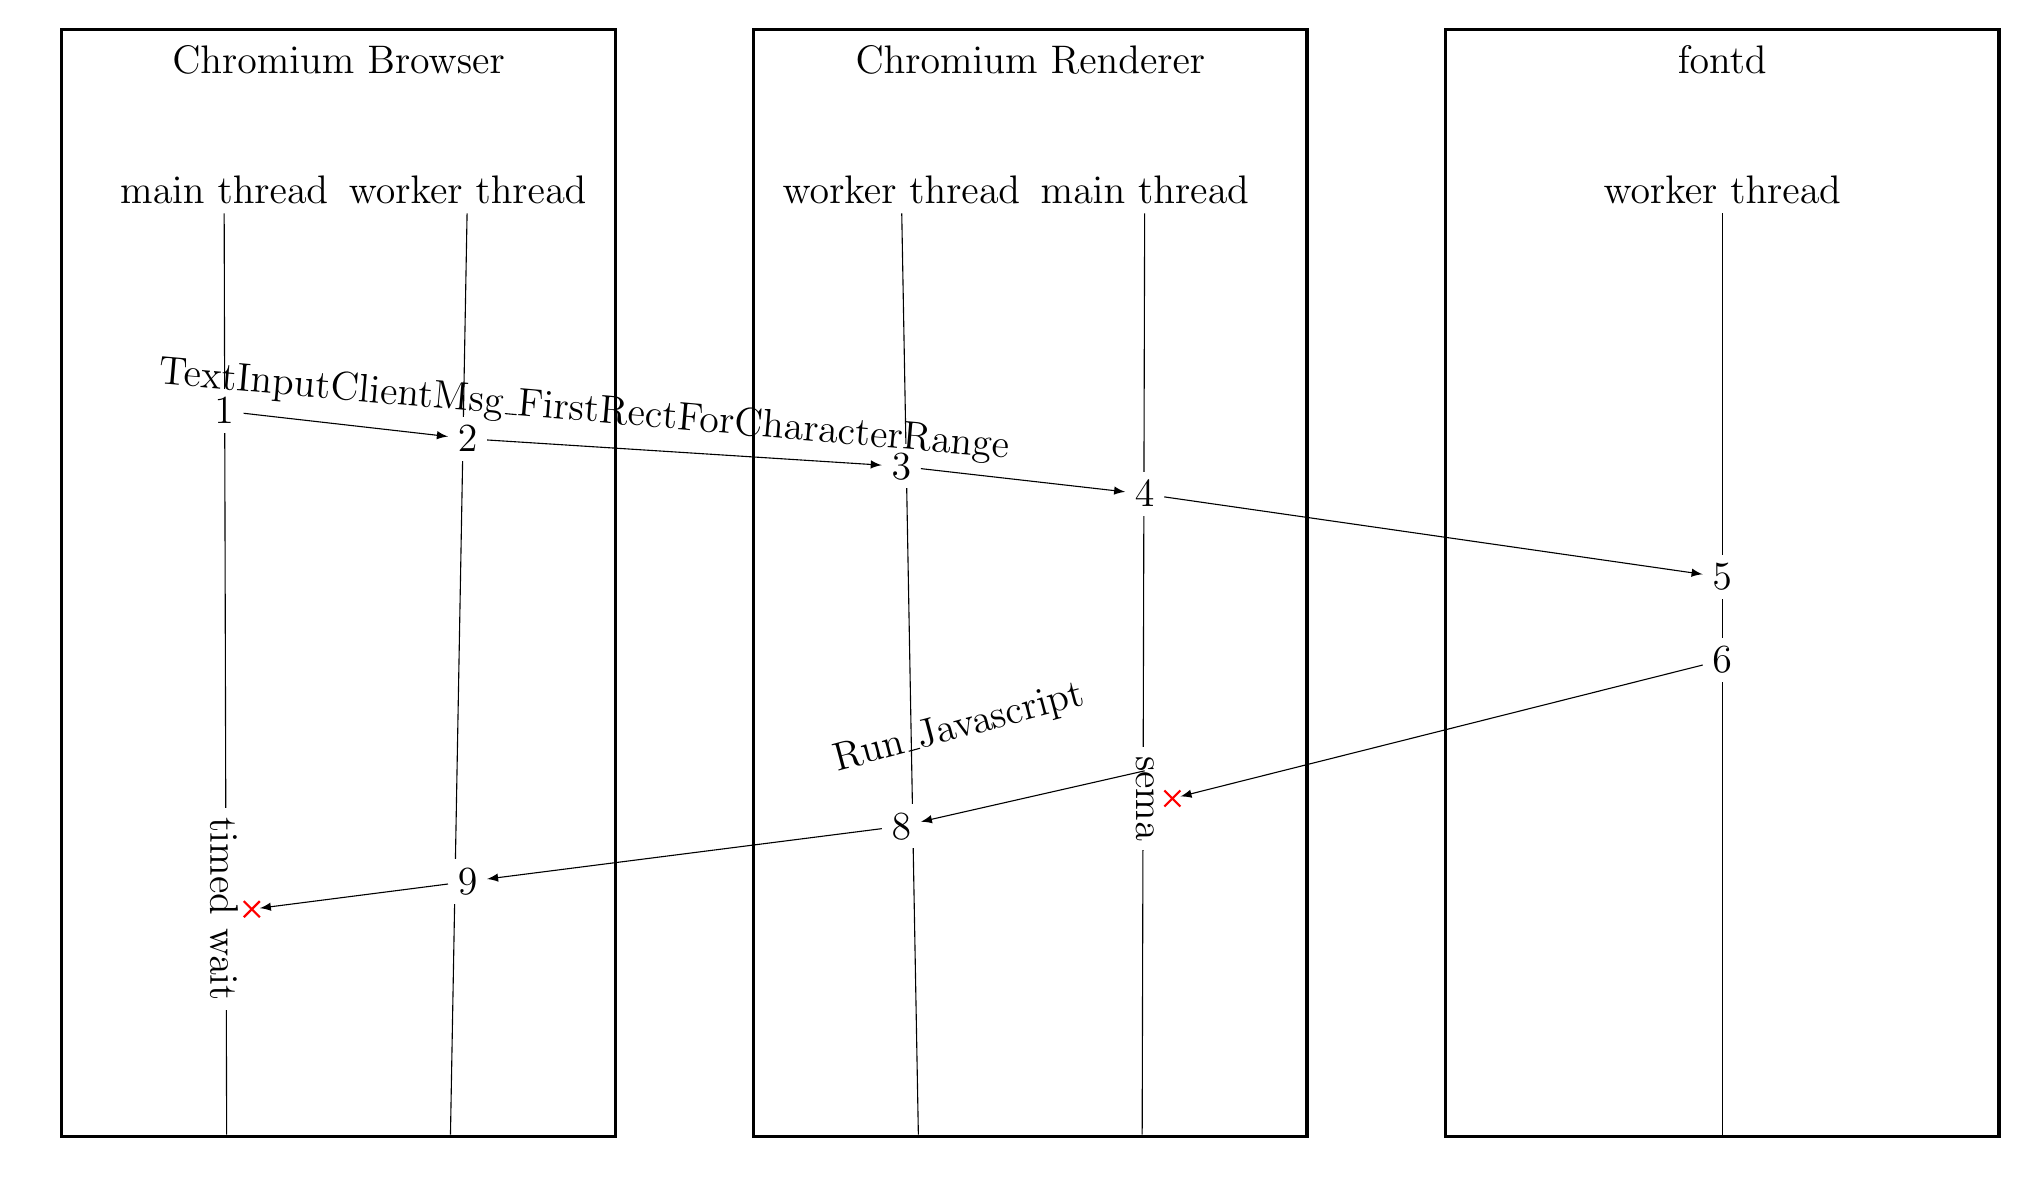
\begin{tikzpicture}[>=latex]
\tikzstyle{every node}=[font=\Large]
\tikzstyle{app} = [draw, very thick, minimum height=40em, minimum width=20em, fill=white, rectangle, font={\sffamily\bfseries}]
\tikzstyle{actionpoint} = [minimum width = 1em, fill = white]
\tikzstyle{point} = [thick, draw=red, cross out, inner sep = 0pt, minimum width = 0.5em, minimum height =0.5em]
%\tikzset{
%%ext/.pic={
%%\path [fill=white] (-0.2,0)to[bend left](0,0.1)to[bend right](0.2,0.2)to(0.2,0)to[bend left](0,-0.1)to[bend right](-0.2,-0.2)--cycle;
%%\draw (-0.2,0)to[bend left](0,0.1)to[bend right](0.2,0.2) (0.2,0)to[bend left](0,-0.1)to[bend right](-0.2,-0.2);
%%},
%point/.style={
%    thick,
%    draw=red,
%    cross out,
%    inner sep=0pt,
%    minimum width=4pt,
%    minimum height=4pt,
%}}

%draw applications
\node [app, name = browser]{};
\node (browsertag)[minimum width = 20em, above = -2em of browser] {Chromium Browser};
\node (browserend)[minimum width = 20em, below = 38em of browsertag] {};
\node (bt1begin)[minimum width = 8em, below left = 3em and -10em of browsertag]{main thread};
\node (bt1end)[minimum width = 8em, below left = 38em and -10em of browsertag]{};
\node (bt2begin)[minimum width = 8em, below right = 3em and -10em of browsertag]{worker thread};
\node (bt2end)[minimum width = 8em, below right = 38em and -10em of browsertag]{};
\draw [solid] (bt1begin) -- (bt1end);
\draw [solid] (bt2begin) -- (bt2end);
\node (1)[actionpoint, below of = bt1begin, node distance = 8em]{1};
\node (2)[actionpoint, below of = bt2begin, node distance = 9em]{2};
\node (9)[actionpoint, below of = 2, node distance = 16em] {9};
\node (10)[actionpoint, below of = 1, minimum width = 6em, minimum height = 2em, node distance = 18em, rotate=270]{timed wait};
%\node (11)[actionpoint, below of = 10, node distance = 4em]{};

\node [app, name = renderer, right of = browser, node distance = 25em]{};
\node (renderertag)[minimum width = 20em, above = -2em of renderer] {Chromium Renderer};
\node (rendererend)[minimum width = 20em, below = 38em of renderertag]{};
\node (bt3begin)[minimum width = 8em, below left = 3em and -10em of renderertag]{worker thread};
\node (bt3end)[minimum width = 8em, below left = 38em and -10em of renderertag]{};
\node (bt4begin)[minimum width = 8em, below right = 3em and -10em of renderertag]{main thread};
\node (bt4end)[minimum width = 8em, below right = 38em and -10em of renderertag]{};
\draw [solid] (bt3begin) -- (bt3end);
\draw [solid] (bt4begin) -- (bt4end);
\node (3)[actionpoint, below of = bt3begin, node distance = 10em]{3};
\node (4)[actionpoint, below of = bt4begin, node distance = 11em]{4};
\node (7)[actionpoint, below of = 4, node distance = 11em, rotate=270] {sema};
\node (8)[actionpoint, below of = 3, node distance = 13em]{8};

\node [app, name = fontd, right of = renderer, node distance = 25em]{};
\node (fontdtag)[minimum width = 20em, above = -2em of fontd] {fontd};
\node (fontdend)[minimum width = 20em, below = 38em of fontdtag]{};
\node (bt5begin)[minimum width = 20em, below = 3em of fontdtag]{worker thread};
\node (bt5end)[minimum width = 20em, below = 38em of fontdtag]{};
\draw [solid] (bt5begin) -- (bt5end);
\node (5)[actionpoint, below of = bt5begin, node distance = 14em] {5};
\node (6)[actionpoint, below of = 5, node distance = 3em] {6};

\draw [->] (1) -- (2);
\draw [->] (2) -- (3);
\draw [->] (3) -- (4);
\draw [->] (4) -- (5);
\coordinate[name = notarrive7, point, right of = 7, node distance = 1em];
\draw [->] (6) -- (notarrive7);
\coordinate[name = before7, above of = 7, node distance = 1em]{};
\draw [->] (before7) -- (8);
\draw [->] (8) -- (9);
\coordinate[name = notarrive10, point, right of = 10, node distance = 1em]{};
\draw [->] (9) -- (notarrive10);

\node (findfirstrect)[minimum width = 40em, minimum height = 4em, right of = 1, node distance = 13em, rotate = 355] {TextInputClientMsg\_FirstRectForCharacterRange};
\node (javascript)[minimum width = 4em, minimum height = 4em, above left = 0em and 2em of 7, rotate = 15] {Run\_Javascript};
\end{tikzpicture}
}
\end{center}
%%\end{document}
 
%%    \caption{Chromium case study.}
%%    \label{fig:chromium-trace}
%%\end{figure*}

Next she ran \xxx to find the event in the main thread of the browser process.
\xxx returned a \vv{cv\_timed\_wait} event %(Figure~\ref{fig:chromium-trace})
that blocked the main thread for a few seconds. Inspection of the
lightweight call stack revealed that this wait happened within a call to
\vv{TextInputClientMac::GetFirstRectForRange}. Without knowing the application's
semantics, she could not understand this method. Thus she ran \xxx to compare
the spinning case to a normal case. \xxx searched in the main thread of the
browser process for vertexes similar to this wait waiting vertexes similar to
this wait, found three, and confirmed with the user which one she wanted.

%%%need to adjust based on the new figure
%%\xxx then found the normal-case wake-up path shown in the figure, which
%%connects five threads.  The browser main thread was signaled by a browser
%%worker thread as shown in step \textcircled{1} of backward slicing in Figure
%%\ref{fig:chromium-trace}, which in turn \vv{read\_file} in step \textcircled{2}
%%for IPC from a worker thread of \vv{renderer}, the daemon for rendering screens.
%%The \vv{renderer} worker thread is woken up by the \vv{renderer} main thread to
%%\vv{read\_file} \textcircled{3}, which in turn \vv{recv\_msg} \textcircled{4}
%%from \vv{fontd}, the font service daemon.  From this path, we could guess that
%%\vv{GetFirstRectForRange} was for the browser to understand the bounding box of
%%the search string.  \xxx further compared the wake-up path with the spinning
%%case, and returned the \vv{wait\_semaphore} event in the \vv{renderer} main
%%thread, the culprit that delayed waking up the browser main thread over 4
%%seconds.

What caused the wait in the \vv{renderer} main thread though?  She thus
continued diagnosis and recursively applied \xxx to the wait in \vv{renderer},
and got the wake-up path shown in the figure for this wait.  Inspection reveal
that the \vv{renderer} requested the browser's help to render Javascript and was
waiting for a reply.  At this point, a circular wait formed because the browser
was waiting for the \vv{renderer} to return the string bounding box and the
\vv{renderer} was waiting for the browser to help render Javascript.  This
circular wait was broken by a timeout in the browser main thread (the
\vv{cv\_timed\_wait} timeout was 1,500 ms).  While the system was able to make
progress, the next key press caused the spinning cursor to display for another
1,500 ms.  The timeout essentially converted a deadlock into a livelock.

\section{Handling Inaccuracies in Causal Tracing}\label{sec:inaccuracy}

\subsection{Inherent Inaccuracies}
%figure dispatch message batching
\begin{figure}[t]
\begin{minipage}[t]{.25\textwidth}
\begin{lstlisting}
//worker thread in fontd:
//enqueue a block
block = dispatch_mig_sevice;
dispatch_async(block);
\end{lstlisting}
\end{minipage}\hfill
\begin{minipage}[t]{.21\textwidth}
\begin{lstlisting}
//main thread in fontd:
//dequeue blocks
block = dequeue();
dispatch_execute(block);
\end{lstlisting}
\end{minipage}

\begin{minipage}[t]{0.48\textwidth}
\begin{lstlisting}
//implementation of dipatch_mig_server
dispatch_mig_server()
for(;;) //batch processing
  mach_msg(send_reply, recv_request)
  call_back(recv_request)
  set_reply(send_reply)
\end{lstlisting}
\end{minipage}
%\vspace{-0.3cm}
    \caption{Dispatch message batching}
    \label{fig:dispatchmessagebatching}
\end{figure}

%figure batching in event processing
\begin{figure}[t]
\begin{lstlisting}
//inside a single thread
while() {
  CGXPostReplyMessage(msg) {
  // send _gOutMsg if it hasn't been sent
    push_out_message(_gOutMsg)
    _gOutMsg = msg
    _gOutMessagePending = 1
  }
  CGXRunOneServicePass() {
    if (_gOutMessagePending)
      mach_msg_overwrite(MSG_SEND | MSG_RECV, _gOutMsg)
    else
      mach_msg(MSG_RECV)
    ... // process received message
  }
}
\end{lstlisting}
%\vspace{-0.7cm}
    \caption{Batching in event processing}
    \label{fig:batchingineventprocessing}
\end{figure}

%% figure coreanimation
\begin{figure}[t!]
\begin{minipage}[t]{.20\textwidth}
\begin{lstlisting}
//Worker thread:
//needs to update UI:
obj->need_display = 1
\end{lstlisting}\hfill
\end{minipage}
\noindent\begin{minipage}[t]{.28\textwidth}
\begin{lstlisting}
//Main thread: 
//traverse all CA objects
if(obj->need_display == 1)
  render(obj)
\end{lstlisting}\hfill
\end{minipage}
%\vspace{-0.7cm}
    \caption{CoreAnimation shared flag}
    \label{fig:casharedflag}
\end{figure}

%%figure spinnin flags
\begin{figure}[t]
\begin{minipage}[t]{0.48\textwidth}
\begin{lstlisting}
//NSEvent thread:
CGEventCreateNextEvent() {
  if (sCGEventIsMainThreadSpinning == 0x0)
     if (sCGEventIsDispatchToMainThread == 0x1)
       CFRunLoopTimerCreateWithHandler{
         if (sCGEventIsDispatchToMainThread == 0x1)
           sCGEventIsMainThreadSpinning = 0x1
           CGSConnectionSetSpinning(0x1);
       }
}
\end{lstlisting}
\end{minipage}
\begin{minipage}[t]{0.48\textwidth}
\begin{lstlisting}
//Main thread:
{
	... //pull events from event queue
	Convert1CGEvent(0x1);
	if (sCGEventIsMainThreadSpinning == 0x1){
  		CGSConnectionSetSpinning(0x0);
  		sCGEventIsMainThreadSpinning = 0x0;
  		sCGEventIsDispatchedToMainThread = 0x0;
	}
}
\end{lstlisting}
\end{minipage}
%\vspace{-0.7cm}
    \caption{Spinning Cursor Shared Flags}
    \label{fig:spinningcursorsharedflags}
\end{figure}


As explained in \S\ref{sec:background}, causal tracing builds a graph to connect
execution segments on behalf of a request that spread across separate threads
and processes. Based on our experience of building a causal tracing system on
commercial closed-source macOS, we believe such graphs are inherently inaccurate
and contain both \emph{over-connections} which do not really map to
causality, and \emph{under-connections}, missing edges between two vertices
with one causally influencing the other. In this section, we present several
inherently inaccurate patterns we observed and their examples.

\subsubsection{Over Connections} \label{subsec:overconnections}

Over connections usually occur when (1) intra-thread boundaries are missing due
to unknown batch processing programming paradigms or (2) superfluous wake-ups
that do not always imply causality.

\paragraph{Dispatch message batching}

While traditional causal tracing assumes the entire execution of a callback
function is on behalf of one request, we found some daemons implement their
service loop inside the callback function and create false dependencies. In the
code snippet in Figure~\ref{fig:dispatchmessagebatching} from the \vv{fontd}
daemon , function \vv{dispatch\_client\_callout} is installed as a callback to
a work from dispatch queue. It subsequently calls \vv{dispatch\_mig\_server()}
which runs the typical server loop and handles messages from different apps. Any
application or daemon can implement its own server loop this way, which makes it
fundamentally difficult to automatically infer event handling boundaries.

\paragraph{Batching in event processing}

Message activities inside a system call are assumed to be related traditionally.
However, to presumably save on kernel boundary crossings, WindowServer MacOS
system daemon uses a single system call to receive data and send data for
an unrelated event from different processed in its event loop in Figure
~\ref{fig:batchingineventprocessing}. This batch processing artificially makes
many events appear dependent.

\paragraph{Mutual exclusion}

In a typical implementation of mutual exclusion, a thread's unlock operation
wakes up a thread waiting in lock. Such a wake-up may be, but is not always,
intended as causality. However, without knowing the developer intent, any
wake-up is typically treated as causality. 

\subsubsection{Under Connections}\label{subsec:underconnections}

We observe that under connections mostly result from missing data
dependencies.  This pattern is more general than shared-memory flags in ad
hoc synchronization~\cite{xiong2010ad} because it occurs even within a
single thread. 

\paragraph{Data dependency in event processing}
The code for Batching in event processing above also illustrates a causal
linkage caused by data dependency in one thread. WindowServer saves the reply
message in variable \vv{\_gOutMsg} inside function \vv{CGXPostReplyMessage}.
When it calls \vv{CGXRunOneServicePass}, it sends out \vv{\_gOutMsg} if there is
any pending message.

\paragraph{CoreAnimation shared flags}
As shown in the code snippet Figure~\ref{fig:casharedflag}, worker thread can set a
field \vv{need\_display} inside a CoreAnimation object whenever the object needs
to be repainted. The main thread iterates over all animation objects and reads
this flag, rendering any such object. This shared-memory communication creates
a dependency between the main thread and the worker so accesses to these field
flags need to be tracked.

%%However, since each object has such a field flag, \xxx cannot afford to monitor
%%each using a watch point register. Instead, it uses instrumentation to modify
%%the CoreAnimation library to trace events on these flags.

\paragraph{Spinning cursor shared flag}
The very fact that spinning cursors are displayed involves data
flags. Each application contains an \vv{NSEvent} thread which fetches
\vv{CoreGraphics} events from the \vv{WindowServer} daemon, converts them
to \vv{NSApp} events to dispatch to the application's main thread, sets
flag \vv{sCGEventIsDispatchToMainThread} as shown in
Figure~\ref{fig:spinningcursorsharedflags}, and arms a timer to monitor
the processing times of the main thread.  If any \vv{NSApp} event takes
longer than two seconds to process, the main thread will not clear flag
\vv{sCGEventIsDispatchToMainThread}.  When the timer in \vv{NSEvent}
fires, it sets flag \vv{sCGEventIsMainThreadSpinning} and invokes
\vv{WindowServer} to display a spinning cursor.  An interesting fact is
that accesses to these shared-memory flags are controlled via a lock --
the lock is used for mutual exclusion, and does not imply a happens before
relationship.

\section{Argus Graph Computing}\label{sec:graphcomputing}

\subsection{Event Graph}\label{subsec:eventgraph}
%%Main point for the subsection: \xxx computes a dependency graph to assist
%%debugging. It is a useful graph to figure out relationships across thread
%%boundary and timing boundary 
%%
%%\begin{itemize}
%%\item What the graph is?
%%
%%	\begin{itemize}
%%	\item Paragraph1: high level description of dependency graph.
%%
%%\xxx constructs dependency graphs with the events from tracing logs. Tracing
%%logs contains sequence of events per thread. Each event stands for an execution
%%step in the thread. They are grouped into nodes and IPCs, asynchronouns calls
%%and thread wakeups serve as edges; some edges can be inside a single thread.
%%
%%	\item Paragraph2: detail about the graph.
%%
%%Events can be classed into three categories: semantic, connection, boundary
%%Graph nodes consist of a list of execution events and edges are generated with
%%event pairs.
%%
%%	\end{itemize}
%%
%%\item Why the graph is userful?
%%The graph bares the causility path of a user input and thus is helpful in
%%debugging complicated performance bugs, which involve mutilple processes and
%%threads.
%%\end{itemize}

\xxx constructs dependency graphs with the events from tracing logs. Tracing
logs contain sequence of events per thread. Each event stands for an execution
step in a thread. They are grouped into nodes and IPCs, asynchronouns calls
and thread wakeups serve as edges; some edges can be inside a single thread.

The events traced in \xxx are carefully selected for three main purposes:
preserve semantics for the node, indentify node boundary inside a thread, and
provide connections between nodes. We classify them into three categories:
semantics events, boundary events and connection events, as listed in
Table~\ref{table:event_types}.

\begin{table}[h]
  \centering
  \begin{tabularx}{\columnwidth}{|X|X|}
  	\hline
    \textbf{Categories} & \textbf{Event types}\\
	\hline
	\hline
    {\bf Semantics Events} & System\_call\\
    provide hints for user & Back\_trace\\					   
	interactive debugging  & NSApp\_event\\
    \hline
    {\bf Boundary Events} & Interrupts\\
	construct nodes & Sharetime\_maintenance\\
	& Wait\\
	& Dispatch\_invoke\\
    & Runloop\_invoke\\
	& Mach\_message\\
    \hline
	{\bf Connection Events} & Wake\_up\\
    add edges & Mach\_message\\
    & Dispatch\_enqueue\\
    & Runloop\_submit\\
	& Share\_flag\_write\\
	& Share\_flag\_read\\
    \hline
  \end{tabularx}
  \caption{Event Type Categories. }
  \label{table:event_types}
\end{table}

Given the prevalent of multi-threading and multi-processing programs, bugs are
much more complicated. The long opening bugs are usually have several threads
involve, even across process boundaries. As an example, the always timeout on
particular synchronization primitive in one thread usually need to trace back to
find the other thread that was responsible for signal on the primitive. Compared
to the existing debugging tools like lldb and spindump, the dependency graph is
useful in that 1) it provides thread relationships all over the system across
processes boundary and timing boundary and 2) it records execution history for
an input event before users capture hangs with their eyes.

\subsection{Inherent Inaccuracy}\label{subsec:inherentinaccuracy}
%%main point: the inaccuracy of causality graph
%%\begin{itemize}
%% 	\item Paragraph1: describe the inaccuracy with general idea, define over
%%connection and under connection
%%
%%	
%%	\item Paragraph2: over connection patterns
%%
%%Over connections occur if intra-thread boundaries are missing from batch
%%processing programming paradigms. (dispatch\_mig\_service, runloop)
%%
%%	\item Paragraph3: under connection patterns
%%
%%Data dependencies inter/intra threads are usually hard to fully exploit in the
%%initial pass of graph computing. (shared flags in Object, data dependency for
%%delay work intra-thread)
%%
%%\end{itemize}

However, to construct an accurate and complete dependency graph is difficult,
if not impossible. The graph is inherently inaccurate. That one thread wakes
up the other thread does not always stand for a causility between them. In
implementation, \xxx filters out some of the definitive noise in the following
types.

%%We identify the purpose of wake-up and add huristics to filter out the false edges.

\begin{itemize}

\item interrupt processing and kernel sharetime maintanance that take over
current thread context.

\item timer expiration in the kernel which clears up all the waiting threads on
an event source.

\end{itemize}

In addition to the known definitive noise, there exist false connections and
miss data dependencies based on our experience while building dependency graph
with traditional causality tracing. We define them as over connection and under
connection respectively.

Over connections occur if intra-thread boundaries are missing from batch
processing programming paradigms. (dispatch\_mig\_service, runloop)

\para{Dispatch message batching}
The message dispatch service dequeues messages from many processes and staggers
processing of the messages. This creates false dependencies between each message
in the dispatch queue. As illustrated in the following code snipped from the
\vv{fontd} daemon, function \vv{dispatch\_execute} is installed as a callback to
a dispatch queue. It subsequently calls \vv{dispatch\_mig\_server()} which runs
the typical server loop and handles many messages.

To avoid incorrectly linking many irrelevant processes through such batching
processing patterns, \xxx adopts the aforementioned heuristics to split an
execution segment when it observes that the segment sends out messages to two
distinct processes. This pattern does pose a challenge for automated causal
tracing tools that assume that the entire execution of a callback function is
on behalf of one request. The code shown uses a dispatch-queue callback, but
inside the callback, it does work on behalf of many different requests. Any
application or daemon can implement its own server loop this way, which makes it
fundamentally difficult to automatically infer event handling boundaries.

{\footnotesize \begin{verbatim}
Worker thread in fontd daemon:
dispatch_async(block)

Main thread in fontd daemon:
block = dispatch_queue.dequeue()
dispatch_execute(block)
  dispatch_mig_server()

dispatch_msg_server()
  for(;;)
    mach_msg(send_reply, recev_request)
    call_back()
    set_reply()
\end{verbatim}
}

\para{Runloop callbacks batch processing}
As is common in event driven programming, many methods can post a callback and
MacOS uses runloop as a common idiom to process callbacks. As shown in the
following step-by-step description of the MacOS runloop, an iteration of the
runloop does 10 different stages of processing, each of which may do work on
behalf of completely irrelevant requests. Since there are no obvious events
(\eg, a wait operation) to split the execution, \xxx uses instrumentation to
add beginning and ending points for MacOS runloops. In general, any application
or daemon can create its own version of the runloop, posing challenges for
automated inference of event processing boundaries.

% // another thread installs cb
% performSelector:onThread:withObject:waitUntilDone;

{\footnotesize \begin{verbatim}
Run loop sequence of events //developer.apple.com
1-3.Notify observers
4.Fire any non-port-based input sources
5.If a port-based input source is ready and waiting to fire,
    process the event immediately. Go to step 9.
6.Notify observers that the thread is about to sleep.
7.Put the thread to sleep until:
    //one of the following events occurs
    An event arrives for a port-based input source.
    A timer fires.
    The timeout value set for the run loop expires.
    The run loop is explicitly woken up.
8.Notify observers that the thread just woke up.
9.Process the pending event.
  If a user-defined timer fired,
    process the timer event
    restart the loop.
    Go to step 2.
  If an input source fired
    deliver the event.
  If the run loop was explicitly woken up, but not timed out,
    restart the loop. Go to step 2.
10.Notify observers that the run loop has exited.

\end{verbatim}
}

\para{Batching and data dependency in event processing}
The WindowServer MacOS system daemon contains an event loop which waits on
Mach messages. Conceptually, it processes a series of independent events from
different processes. However, to presumably save on kernel boundary crossings,
it uses a single system call to receive data and send data for an unrelated
event. This batch processing artificially makes many events appear dependent,
and we split the execution segments to maintain the independence of the events.

This case also illustrates a causal linkage caused by data dependency within
one thread. As the code shows, WindowServer saves the reply message in variable
\vv{\_gOutMsg} inside function \vv{CGXPostReplyMessage}. When it calls
\vv{CGXRunOneServicePass}, it sends out \vv{\_gOutMsg} if there is any pending
message. This data dependency needs to be captured in order to establish a
causal link between the handling of the previous request and the send of the
reply. Interestingly, it is an example of a data dependency within the same
thread. \xxx uses watch point registers to capture events on these data flags
and establish causal links between them.

{\footnotesize \begin{verbatim}
while() {
  CGXPostReplyMessage(msg) {
  // send _gOutMsg if it hasn't been sent
    push_out_message(_gOutMsg)
    _gOutMsg = msg
    _gOutMessagePending = 1
  }
  CGXRunOneServicePass() {
    if (_gOutMessagePending)
      mach_msg_overwrite(MSG_SEND | MSG_RECV, _gOutMsg)
    else
      mach_msg(MSG_RECV)
    ... // process received message
  }
}
\end{verbatim}
}

Under connections are result from particular programing paradigms and data
dependencies. Data dependencies inter/intra threads are usually hard to fully
exploit in the initial pass of graph computing. (shared flags in Object, data
dependency for delay work intra-thread)

\para{CoreAnimation shared flags}
A worker thread can set a field \vv{need\_display} inside a CoreAnimation object
whenever the object needs to be repainted. The main thread iterates over all
animation objects and reads this flag, rendering any such object.

This shared-memory communication creates a dependency between the main thread
and the worker so accesses to these field flags need to be tracked. However,
since each object has such a field flag, \xxx cannot afford to monitor each
using a watch point register. Instead, it uses instrumentation to modify the
CoreAnimation library to trace events on these flags.

{\footnotesize \begin{verbatim}
Worker thread that needs to update UI:
ObjCoreAnimation->need_display = 1

Main thread: 
traverse all CoreAnimationobjects
if (obj->need_display == 1)
  render(obj)

\end{verbatim}
}

\para{Spinning cursor shared flag}
Whenever the system determines that the main thread has hung for a certain
period, and the spinning beach ball should be displayed, a shared-memory flag
is set. Access to this flag is controlled via a lock, i.e. the lock is used for
mutual exclusion, and does not imply a happens before relationship. Thus, \xxx
captures accesses to these flags using watch-point registers to add causal edges
correctly.

{\footnotesize \begin{verbatim}
NSEvent thread:
CGEventCreateNextEvent() {
  if (sCGEventIsMainThreadSpinning == 0x0)
     if (sCGEventIsDispatchToMainThread == 0x1)
       CFRunLoopTimerCreateWithHandler{
         if (sCGEventIsDispatchToMainThread == 0x1)
           sCGEventIsMainThreadSpinning = 0x1
           CGSConnectionSetSpinning(0x1);
       }
}

Main thread
Convert1CGEvent(0x1);
if (sCGEventIsMainThreadSpinning == 0x1)
  CGSConnectionSetSpinning(0x0);
  sCGEventIsMainThreadSpinning = 0x0;
  sCGEventIsDispatchedToMainThread = 0x0;
\end{verbatim}
}

In addition, the spurious edge introduced by mutex lock is also a challenge in
debugging. The synchronization on mutex lock reflects one thread wakes up the
other thread. They can depend on each other like producer and comsumer, while
no causality exists in the case of contention for a shared resource. Making the
graph completely sound without user interaction is almost impossible given the
essential attribite of commericial operating system as a grey box.

\subsection{User Interactions}

%%Main point for the subsection: why we need user interaction, what the user can
%%do and how it helps
%% Para1 : why we need user interaction
%% Para2 : what the user can do
%% Para3 : how it helps causality tracing

As we mentioned above, to figure out all the over connections and under
connections before hand is almost impossible. Instead, users can find out the
descrepency on the dependency graph while checking the computing result. For
example, we noticed that two unrelated applications connects to one node in the
graph, which leads to the manifestation of kernel thread batch processing on
timers. Users can gradually inject their knowledge until the graph is reasonable
for following debugging.

Over connections in this kind can be eliminated by adding heuristics to the
process of graph computing. In addition, users can also binary instrument the
image with the APIs provided by \xxx to amending the missing boundaries. On
contrary, if users discover under connections due to missing data dependency,
they can make use of the \xxx's hardware breakpointer tool to monitor the data
and add rules to recompute the graph.

Like other causality tracing approaches, \xxx is a general framework and tested
on limited data set. Allowing user interaction makes the dependency graph more
practical and useful case by case.

\subsection{Graph Computing Algorithm}

In the section, we describe the algorithm \xxx used to generate an event graph.
The algrithm has two main steps: construct nodes with heuristics base on
boundary events, and generate edges from the connection events.

A node is a sequence of events derived from the execution of a task in a thread.
As is shown in Figure ~\ref{fig:alg-graphcomputing}, \xxx checks events per
thread and applies heuristics when a boundary event is encoutered. \xxx provides
5 default heuristics. 4 of them shares the idea of general cuasual tracing, 1
is used to work around unknown programming pargdigms, and more are expected
from users to improve graphs. We discuss them in the following paragraph.

As known noises, event sequences for interrupt processing and kernel
maintainance are removed from threads, as is shown in 1.a. The second heuristics
1.b treats a wait event as an end of node. Wait event usually indicates a thread
switches to other tasks, but it is not always true considering a thread may park
due to low thread priority. One of the examples in MacOS is the pause of worker
threads draining a low priority diapatch queue. Dispatch queues are FIFO queues
to which an application can submit tasks in the form of block objects. Wait
events should not divide the block objects, otherwise it may result in a missing
connection. To save the intergrity of block objects, \xxx GraphComputeAlgorithm
keeps a counter \vv{callout\_level} to mark if the currently checking event is
inside a block object. Only the begin and end of Dispatch\_invoke are served
as the boundary for the node, as is shown in the step 1.c. The hueristics 1.d
is also for a batch processing mechanism. Runloop is an event processing loop
that used to schedule work and coordinate the receipt of incoming events.
The begin and end of the work invocation are served as boundaries. The last
default heuristics 1.e is used to work around the problem that batch processing
programming paragdigms are hard to exploit completely, as listed in previous
subsection ~\ref{subsec:inherentinaccuracy}. \xxx makes use of mach messages
to avoid clustering multiple tasks due to unknown batch processing. It defines
\vv{IPC\_peer\_set} to compute the set of mach message receivers/senders for
every node. For every mach message, the algorithm checks whether its peer
process exists in \vv{IPC\_peer\_set}, and adds the message into the current
node if the condition is true or the set is empty. Otherwise it add a boundary
for current node and begin a new node for the mach\_message event.

Edges connect nodes, both intra-thread and iter-thread, with connection events.
\xxx walks through each connection event types to apply heuritics as follows.
First, the return from a wait operation causally depends on the wake-up
operation. An edge is defined from the wake-up event to the first event after
the wait returns. \xxx also add a weak edges from the wait event to the wake-up
event in 2.a. Mach message is the core of ipc mechanism implemented in kernel,
upon which higher level RPC are built. \xxx connects the sender and receiver
of a mach message. For messages that expect a reply, \xxx also connects the
receiver of the original message and the sender of the reply message in 2.b.
As discussed above, dispatch queue and runloop are popular batch processing
programming paradigms in MacOS, \xxx connects submissions of a task and
executions of the task, which are listed in 2.c and 2.d respectively. Similarly,
\xxx adds edge from a timer armed event to its triggered event in 2.e. Shared
flag can either be traced with binary instrument, such as \vv{need\_display}
flag for CoreAnimation in subsection ~\ref{subsect:inherentinaccuracy}, or with
breakpoint watcher command line tool provided by \xxx. Edges from the flag set
to its read are added as 2.f. Since share variables are hard to completely
exploited, and the causality can be complicated than the writer-reader pattern,
user interaction are expected to remedy event graphs.

Finally, the computing graph is generated and subject to the improvement with
more input heuristics.

\begin{figure}[tb]
\footnotesize\begin{verbatim}
Algorithm ComputeControlFlowGraph:
    Input: Heuristics set + parsed tracing events
    Output: Control flow graph
1. Create nodes per thread:
  set callout_level = 0
  1.a interrupt/kern_maintainance: remove_events
  1.b wait: end of node if callout_level == 0
  1.c if dispatch_callout begin, create a new node
      and increase callout_level
      if dispatch_callout end, complete current node
      and decrease callout_level
  1.d Runloop: divide every callout
  1.e mach_msg: divide IPC with different peers
  1.f Other heuristics added by user from the input set.
2. Add edges for connection events:
  2.a wake_up event and wait event
  	edge(wake_up, first_waken_event)
	weak_edge(wait, wake_up)
  2.b mach message
  	edge(sender, receiver)
    if message needs reply
       edge(receiver, reply_sender)
  2.c dispatch queue events
  	edge(work_enqueue, work_dequeue)
  2.d Runloop work submission
  	edge(work_submit, work_invoke)
  2.e timer events
  	edge(timer_armed, timer_fired)
  2.f shared variable
  	edge(set_variable, read_and_clear_variable)
  2.g Other heuristics added by user from the input set.
3. Return the Graph with Nodes and Edges
\end{verbatim}
    \caption{\xxx Compute Graph algorithm.}
    \label{fig:alg-graphcomputing}
\end{figure}

\section{Implementation}\label{sec:implementation}
We now discuss how we collect tracing events from both kernel and libraries.

\subsection{Event Tracing}

Current MacOS systems support a system-wide tracing infrastructure built by
Apple ~\ref{linktotracetool}. By default, the infrastructure temporarily stores
events in memory and flushes them to screen or disk when an internal buffer is
filled. We extended this infrastructure to support larger-scale tests and avoid
filling up the disk with a file backed ring buffer. Subject to configurarion,
it allows at most 2GB of data per log, which corresponds to approximately
18,560,187 events (about 5 minute with normal operations).

The default tracing points in MacOS do not provide enough information to
generate a dependency graph. As a result, we both patch source code of kernel
and binary instrument libraries to gether more tracing information.

\subsection{Instrumentation}

On MacOS, most libraries as well as many of the applications used day-to-day are
closed-source. To add tracing points to such code, techniques such as library
preloading to override individual functions are not applicable on MacOS, as
libraries use two-level executable namespaces~\cite{}. Hence, we implemented
a binary instrumentation mechanism that allows developers to add tracing at
any location in a binary image. Like Detour~\cite{hunt1999detours}, we use
static analysis to decide which instrumentation to perform, and then enact this
instrumentation at runtime.

%XXX I thought a user can specify a search sequence of instructions, and our
%system adds instrumentation when the sequence is found in binary.  If so we
%want to emphasize it a bit as this feature is different from detour.
%XXX say that instrumentation code is written in C
In \xxx, we patched the kernel with 1193 lines of code, and instrumented
the libraries including: libsystem\_kernel.dylib, libdispatch.dylib,
libpthread.dylib, CoreFoundation, CoreGraphics, HIToolbox, AppKit and QuartzCore,
with our binary instrumentation. 

Now we talk about our instrumentation mechanism. Firstly, users find a location
of interest in the image related to a specific event by searching a sequence of
instructions. Then the users replace a call instruction to invokes a trampoline
target function, in which we overwrite the victimed instructions and produce
tracing data with API from Apple. All of the trampoline functions are grouped
into a new image, as well as an initialization function which carries out the
drop-in replacement. Then command tools from \xxx helps to configure the image
with the following steps: (1)re-export all symbols from the original image so
that the original code can be called Like an shared library; (2)replace the
original image with the new one by renaming them to ensure the modifications
are properly loaded; (3)invoke the initialization function externally through
\texttt{dispatch\_once} during the loading.

%%One potential issue is that we use 5-byte call instructions with 32-bit
%%displacements to jump from the original library to our new one.  This design
%%requires that the libraries be loaded within +/- 2GB of each other in the
%%64-bit process address space.  However, since we list each original library as
%%a dependency of our new libraries, the system loader will map each new and
%%original library in sequence.  In practice, the libraries ended up very close
%%to one another and we did not see the need to implement a more general
%%long-jump mechanism.

%%\subsection{Tracing Custom Primitives} \label{subsec:tcp}
\subsection{User Interaction} \label{subsec:tcp}

%%XXX give a simple command line example of how a user can ask \xxx to trace a
%%data flag
%%XXX say what we do in watch point exception handler (record instruction so
%%can determine read or write, and reg values)

As described in (\S\ref{subsec:userinteraction}), under-connection due to
the missing share data dependency requires users'interaction. \xxx provides
a command line tools to record the share\_flag\_write and share\_flag\_read
events in ad-hoc manner. The tool takes the process id, path to image where the
variable is defined and the symbol of the variable as input. We show the simple
example how a user ask \xxx to trace \_gOutMsgPending in the following command.

\begin{BVerbatim}
./bp_watch pidofWindowServer \
	Path/to/CoreGraphics _gOutMsgPending
\end{BVerbatim}

\xxx hooks the watch point handler in CoreFoundation to make sure that it is
loaded correctly into the address space of our target application. The handler
invokes the event tracing API from Apple to record the value of the shared
variable and the operation type: read or write.

\subsection{Capturing Instructions for Diagnosis}

%XXX Talk about what data we gather using lldb, the debugger in the LLVM compiler tool chain.

After the offline analysis on the graph, we take the API covers the fine range
as input to our debugging scripts.  The debugging scripts go throught the
instruction from application and higher level frameworks step by step.  The
purpose is to capture the parameters results from the user interaction.  Once a
new function begins by checking the instruction, we record the call stacks for
comprehension.  For API from the low level libraries, such as pthread, we step
over and record the return value. The debugging log in this step records the
instruction and its address, callstacks when a \textit{call} instruction is reached,
and return values of \textit{req} instruction. As the operation are confined in the
small range, the overhead is not too much.

Both the execution on normal case and problematic case are recorded, our tool
further compares the log and report the difference, with the full call stack.

%%\subsection{Finding Similar Events}
%%
%%The performance isssue caused by the busy processing in UI thread is quite
%%straightforward to diagnoze with our tool. Debugging the UI thread blocking on
%%the contention of resource is much more difficult.  In this situation, our tool
%%is required to recognize the corresponding node which obtained the resource in
%%its normal execution.
%%
%%Node comparision algorithm helps to allieviate users from the burden of
%%inspecting large logs.  We first normalize the nodes with selected events.  In
%%our system, we exclude the interrupts from the comparison since the number and
%%type of interrupts are usually different from execution to exection.  For the
%%events that connected to other events, we normalize it with a peer attribute to
%%record the process id of its connecting peer, We also record the name of the
%%system calls, message id carried in mach\_msg for corresponding events.  The
%%comparison algorithm omits the repeating times of the same events, by checking
%%if one node contains all distinct events in the other node.
%%
%%The above step only idenfity the similarity of nodes.  We also define the
%%differential attribtes to distinguish the normal node and spinning node,
%%including the waiting time, execution time and system call return values.

\subsection{Case Studies}\label{sec:casestudy}

In this section, we demonstrate how \xxx helps to diagnose \nbug
spinning-cursor cases in popular applications. Table~\ref{table:bugs-desc}
describes these spinning-cursor cases.

In Table~\ref{table:results}, we compare \xxx with Panappticon and list the
portions of over- and under- connections disclosed.
However, the filtered graph remains too inaccurate to automate diagnosis. 
%interactions help the path slicing while not overwhelming in the diagnosis
%process.  Our results in Table~\ref{table:results} show
%Paths sliced by \xxx are shorter and easier to inspect.
The user interaction is still required but not overwhelming. In most cases, up
to 3 user queries suffice to find root cause path accurately. Although complex
applications like MicosoftWord and Chromium require more queries, 13 and 22
respectively, many of them result from repeated patterns. They can be easily
identified by users.

Overall, in the case of simple text editing applications, \xxx can identify the
UI event that causes a spinning cursor by merely relying on a few heuristics.
However, these heuristics may make the wrong decision in complicated cases, and
misidentify the relationships between intra/inter-thread events. It is unlikely
that there exists a single graph search method that works in all cases, e.g.
when given the choice between multiple incoming edges, the most recent match is
sometimes correct, but sometimes not. This is why our system relies on expert
knowledge of users to reconstruct a developer's intent and accurately diagnose
performance issues.

%TableXXX describes these spinning-cursor cases.
%Should have a table for issue description
%Bug ID |  Application  |  Bug Description
\begin{table}[t]
\footnotesize
\centering
  \begin{tabularx}{\columnwidth}{l|cl}
    \hline
    \textbf{Bug ID} & \textbf{Application} & \textbf{Bug description}\\
    \hline
	\hline
	 0-Chormium & Chormium & \begin{tabular}{@{}l@{}}
	 Typing non-english in search box\\
	 causes webpage freeze.
	 \end{tabular}
	 \\
     \hline
	 1-SystemPref & \begin{tabular}{@{}l@{}} 
	 System Preferences\\
	 \end{tabular}
	 & \begin{tabular}{@{}l@{}}
	 Disabling an online external mo-\\
	 nitor and rearranging windows\\
	 causes System Preferences freeze.\\
	 \end{tabular}
	 \\
     \hline
	 2-SequelPro& \begin{tabular}{@{}l@{}} 
	 Sequel Pro
	 \end{tabular}
	 & \begin{tabular}{@{}l@{}}
	 Lost connection freezes the APP.
	 \end{tabular}
	 \\
     \hline
	 3-TexStudio & \begin{tabular}{@{}l@{}} 
	 TeXStudio
	 %: LaTeX editor
	 \end{tabular}
	 & \begin{tabular}{@{}l@{}}
	 Modification on bib file with vim\\
	 causes its main window hang.
	 \end{tabular}
	 \\
     \hline
	 4-Installer & \begin{tabular}{@{}l@{}} 
	 Installer
	 \end{tabular}
	 & \begin{tabular}{@{}l@{}}
	 Moving cursor out of an authenti-\\
	 cation window causes freeze.
	 \end{tabular}
	 \\
     \hline
	 5-Notes& \begin{tabular}{@{}l@{}} 
	 Notes\\
	 \end{tabular}
	 & \begin{tabular}{@{}l@{}}
	 Launching Notes where stores a\\
	 long note before causes freeze.
	 \end{tabular}
	 \\
     \hline
	 6-TextEdit & \begin{tabular}{@{}l@{}}
	 TextEdit
	 \end{tabular}
	 & \begin{tabular}{@{}l@{}}
	 Copying text over 30M causes\\
	 freeze.
	 \end{tabular}
	 \\
     \hline
	 7-MSWord & \begin{tabular}{@{}l@{}}
	 Microsoft Words
	 \end{tabular}
	 & \begin{tabular}{@{}l@{}}
	 Copying a document over 400 pa-\\
	 ges causes hang.
	 \end{tabular}
	 \\
     \hline
	 8-SlText & Sublime Text
	 & \begin{tabular}{@{}l@{}}
	 Copying in a file over 49000 lines\\
	 causes freeze.
	 \end{tabular}
	\\
    \hline
	 9-TextMate & TextMate 
	 & \begin{tabular}{@{}l@{}}
	 Pating text over 4000 lines causes\\
	 freeze.
	 \end{tabular}
	\\
    \hline
	 10-CotEditor & CotEditor
	 & \begin{tabular}{@{}l@{}}
	 Pasting in file with 4000 lines co-\\
	 ntext causes freeze.\\
	 \end{tabular}
	\\
	 \hline
  \end{tabularx}
 	\parbox{\columnwidth}{\caption{Bug Descriptions. We assign each bug in Column \textbf{Bug ID} to ease discussion}
  	\label{table:bugs-desc}
  	}
\end{table}


%Bug 0-Apple is ...... The spinning cursor is created when the main thread
%stops responding to events for two seconds. Every application has an
%NSEvent thread, which coordinates with WindowsServer to display a spinning
%cursor when necessary. Two data flags ``\vv{is\_mainthread\_spinning}'' and
%``\vv{dispatch\_to\_mainthread}'' are involved.
%Start a new paragraph "TableXXX shows the results. [Here we should show the big
%table, and talk about the high-level bits.]"

\begin{table*}[ht]
\footnotesize
\centering
  \begin{tabularx}{\textwidth}{l|ccccccc}
 	   & \% of & \% of & \# of& \# of & \multicolumn{2}{c}{size of baseline/spinning path}& auto slicing\\
       & connections & connections added  & user provided & user  & \multicolumn{2}{c}{with}  & over \\
Bug ID & filtered out & by heuristics & data flag & interactions & interactive slicing & automatic slicing &  interactive slicing\\
\hline
\hline
1-Chromium & 0.02 & 0.02 & 0 & 13 & 32 & 303 & 9.47\\
2-SystemPref & 0.56 & 2.48 & 2 & 1 & 2 & 30 & 15.00\\
3-SequelPro & 0.49 & 0.35 & 0 & 2 & 5 & 264 & 52.80\\
4-Installer & 4.39 & 2.83 & 0 & 2 & 6 & 36  & 6.00\\
5-TeXStudio & 2.43 & 0.58 & 0 & 3 & 6 & 44  & 7.33\\
6-Notes & 2.97 & 11.53 & 0 & 2 & 10 & 42 & 4.20\\
7-TextEdit & 7.97 & 0.72 & 0 & 3 & 21 & 21 & 1.00\\
8-MSWord & 6.72 & 1.04 & 0 & 22 & 67 & 136 & 2.03\\
9-SlText & 4.07 & 0.92 & 0 & 1 & 3 & 3 & 1.00\\
10-TextMate & 2.15 & 2.18 & 0 & 0 & 3 & 3 & 1.00\\
11-CotEditor & 4.81 & 5.32 & 0 & 1 & 4 & 6 & 1.50\\

\hline
  \end{tabularx}

  \parbox{\textwidth}
  {\caption{Graph Comparison} 
	  %{1.\xxx filters out connections by dividing a batch processing vertex into
		%  vertices, and adds connections as edges for data flag or heuristic. The portion
		%  changed is small. 2.\xxx only requires a few user interactions, but it is
		%  critical to reduce the path, so as to reduce user's inspecting efforts in
		%  diagnosis. 3.The last column shows the ratio of path size with user interactions
    %over the automatic slicing.}
    {The first and second columns present the portions of over-/under-connections mitigated by \xxx compared
     to traditional cuasal tracing. Column 3 shows the number of data flag added for diagnosis
     in addition to the default data flags \xxx tracks. The forth and fifth columns illustrate
     the numbers of vetices in backward slicing causal paths, with and without user interaction.
     The last column shows how many times the size of path would grow without user interactions.
	 Even after being filterd by \xxx heuristics,they still includes too much vertices for inspection.
    }
  \label{table:results}
  }

\end{table*}
%Last paragraph:
%In the remaining of this section, we present the case studies by category in (\S\ref{XXX}). 
\subsection{Long Wait and Repeated Yield}

In this section, we discuss the cases where the \spinningnode is blocking on
wait event or yielding loop, corresponding to Long Wait and Repeated Yield.

\paragraph{2-SystemPref}

System Preferences provides a central location in macOS to customize system
settings, including configuring additional monitors. A tool called
\vv{DisableMonitor}~\cite{disablemonitor} provides full functionality including
the ability to enable/disable monitors online. We blocked on the spinning
cursor while disabling an external monitor and rearranging windows in
\vv{Display} panel.

The log collected with \xxx contains 1) a baseline scenario where the displays
are rearranged with the enabled external monitor, and 2) a spinning scenario in
which we disable the external monitor with \vv{DisableMonitor} and rearrange
the displays. The \spinningnode in the main thread is dominated by system
calls, \vv{mach\_msg} and \vv{thread\_switch}, which falls into the category of
Repeated Yield. We discovered two missing data flags with \vv{lldb},
``\vv{\_gCGWillReconfigureSeen}'' and ``\vv{\_gCGDidReconfigureSeen}'', which
signify the configuration status and break the thread-yield loop. \xxx learns
from the baseline scenario that the main thread is responsible to set both of
them after receiving specific datagrams from WindowServer. Conversely, the
setting of ``\vv{\_gCGDidReconfigureSeen}'' is missing in the spinning case,
where the main thread yields repeatedly to send messages to WindowServer for
such datagram.

In conclusion, we discovered that the bug is inherent in the design of the
CoreGraphics library, and would have to be fixed by Apple. We verified this
diagnosis by creating a dynamic binary patch with lldb to fix the deadlock. The
patched library makes DisableMonitor work correctly, while preserving correct
behavior for other applications.

\paragraph{3-SequelPro}

Sequel Pro~\cite{SequelPro} is a fast, easy-to-use Mac database management
application for working with MySQL. It allows user to connect to database with
a standard way, socket or ssh.

We experienced the non-responsiveness of Sequel Pro when it lost network
connection and tried reconnections. The tracing data collected by
\xxx contains 1) a quick network connection during login, and 2) Sequel Pro
lost connection for a while. Although \xxx identified the \spinningnode and
corresponding (baseline) \similarnode with ease, it cannot get the correct
causal path in the baseline scenario without user interaction. The backward
slicing on vertex has multiple incoming edges, including one from a kernel
thread, which means that operations are likely to be batched together and
inseparable by heuristics. Our interactively search is extremely helpful in
this step, greatly reducing the noise in the path. Close examination of the
\spinningnode based on the causal path tells us that the main thread is waiting
for the kernel thread, which in turn waits for the ssh thread. Existing
debugging tools like \vv{lldb} and \vv{spindump} cannot determine the root
cause, because both of them diagnose with only call stacks, missing the
dependency across processes.

\paragraph{4-Installer}

Installer~\cite{Installer} is an application included in macOS that extracts
and installs files out of \vv{.pkg} packages. When \vv{Installer} pops up a
window for privileged permission during the installation of
\vv{jdk-7u80-macosx-x64}, moving the cursor out of the popup window triggers a
spinning cursor.

As we put in the password before the round of triggering the spinning cursor,
\xxx successfully records the baseline scenario. Examining the \spinningnode
and its \similarnode, \xxx figures out the daemon \vv{authd} blocks on
semaphore while the main thread is waiting for \vv{authd}. Further checking on
\vv{authd}, \xxx reveals it is the \vv{SecurityAgent} that processes user input
and wakes up \vv{authd} in baseline scenario. In conclusion, moving the mouse
out of the authentication window causes the missing edge from
\vv{SecurityAgent} to \vv{authd}, which in turn blocks \vv{Installer}.

We also discovered a communication pattern in \vv{Installer} underpinning the
crucial of interactive debugging. It involves four vertices in four threads,
vertex $Vertex_{main}$ in the main thread, and $Vertex_1$ to $Vertex_3$ in
three worker threads. First, the main thread wakes up three worker threads.
Then one worker thread is scheduled to run. At its end, another worker thread,
which waits on mutex lock, is woken in $Vertex_2$, which in turn wakes up the
next worker thread in $Vertex_3$. While \xxx is slicing backward, $Vertex_3$
has two incoming edges: one is from $Vertex_{main}$, and the other one is from
$Vertex_2$. Since users can peek the edges before making decision, they are
likely to figure out that the three worker threads contend with mutex lock, and
all of them are successors of $Vertex_{main}$.


\subsection{Long Running}

In this section, we discuss the cases where the \spinningnode is busy on the
CPU. Most of the text editing apps fall into this bug category. We studied
TeXstudio, TextEdit, Microsoft Word, Sublime Text, Text Mate and CotEditor to
reveal their root causes.

%represent cases in this category.

\paragraph{3-TeXStudio}

TeXstudio~\cite{TeXStudio} is an integrated writing environment for creating
LaTeX documents. We noticed a user reported spinning cursor when he
modified his bib file. Although the issue was closed by the developer, due to
insufficient information to reproduce the bug, we reproduced it with a large bib
file opened in a tab. Each time we touched the file through another editor, vim
for example, the application window showed a spinning cursor.

\xxx recognizes the \spinningnode belongs to the category of \textbf{Long
Running}. Slicing causal path from the vertex, \xxx reaches daemon
``\vv{fseventd}'' and figures out that the long-running function is invoked by a callback
function from this daemon. The advantage of \xxx over other debugging tools is
it helps to narrow down the root cause with the path. If the user's bug report
had included details captured with \xxx, it may have provided the developer with
enough information to reproduce the bug successfully.

\paragraph{6-TextEdit}

TexEdit is a simple word processing and text editing tool shipped by Apple, which
often hangs on the editing of large files. 

\xxx reveals the same causal path with heuristics as with user
interaction. We observed a communicating pattern in the vertices where a kernel
thread was woken up from blocking IO by another kernel thread; and it processed
the timer armed by TextEdit and woke up one of its threads. The first incoming
edge is from the second kernel thread, and the second incoming edge is from
TextEdit(from vertex where the timer armed to where it is processed). Users can
make decision on the vertex base on the event sequence, which implies the story:
TextEdit first arms the timer for IO work, then kernel threads work for it, and
finally it processes the timer and wakes up TextEdit when finished.

It is not surprising because the pattern of vetices in the case fits the
hueristics in \xxx, which chooses the most recent incomming edge.
Although the automatic heuristics works for the particular simple tool, it is
not general enough to make decision for all patterns on complex softwares.

\paragraph{7-MSWord}

Microsoft Word is a large and complex piece of software. \xxx can analyze the
event graph, but it identifies multiple possible root causes: the length of path
interactively sliced from the \spinningnode is 67, while the automatic slicing
generates a path of 136 vertices.

%We rely on user interactions to help speed up the path slicing.

We compared the path and find that the earliest difference exists in the
predecessor of the third vertex in backward paths. In the vertex, user
can learn from the callstack that \vv{Microsoft Word} launches a service
\vv{NSServiceControllerCopyServiceDictionarie} after being woken by another
\vv{Microsoft Word} thread; this thread then sends a message to \vv{launchd}
to register the new service and waits for a reply message. With the most
recent edge heuristics in automatic slicing, \xxx chose \vv{launchd} as its
precedessor, but the user can more precisely identify that the execution segment
is on behalf of the first thread. We rely on user interaction in this case
to find the true root cause, since \xxx has identified multiple
possibilities.

\paragraph{Other Editing Apps}

Select, copy, paste, delete, insert and save are common operations for text
editing. However, these operations on a large context usually trigger spinning
cursors. Depending on their implementations, CotEditor and TextMate successfully
avoid hangs on copy and selection operation. \xxx can helps the developer to
figure out the more efficient way to implement event handlers. We briefly list
the reports from \spinningnode, including the event handler and most costly
functions. We also list corresponding user input event from the path slicing in
Table~\ref{table:texteditapps}.

\begin{table}[H]
\vspace{-0.2cm}
\footnotesize
\centering
  \begin{tabularx}{\columnwidth}{l|l|l}
  \hline
  \hline
                  &                     &\\
  \textbf{BUG-ID} & \textbf{costly API} &UI\\
  \hline
  \hline
  5-Notes         & \begin{tabular}{@{}l@{}}
  					\vv{1)NSDetectScrollDevices}\\
					\vv{\xspace ThenInvokeOnMainQueue}\\
					\end{tabular}
   		          & \begin{tabular}{@{}l@{}}
				  	\vv{system}\\
					\vv{define}\\
					\vv{event}
					\end{tabular}
				  \\
  \hline
  6-TexEdit       & \begin{tabular}{@{}l@{}}
  					\vv{1)[NSTextView(NSPasteboard) \_write}\\
					\vv{\xspace RTFDInRanges:toPasteboard:]}\\
					\vv{2)get\_vImage\_converter}\\
  					\vv{3)get\_full\_conversion\_code\_fragment}\\
					\end{tabular}
				  & \vv{key c}
				  \\
  \hline
  7-MSWord        & \begin{tabular}{@{}l@{}}
					\vv{1)-[NSPasteboard setData:}\\
					\vv{\xspace forType:index:usesPboardTypes:]}\\
 					\vv{2)\_CFStringCreateImmutableFunnel3}\\
  					\vv{3)platform\_memmove}\\
					\vv{4)lseek}, \vv{5)fstat64}, \vv{6)fcntl}\\
					\end{tabular}
				  & \vv{key c}
				  \\
  \hline
  8-SlText   & \begin{tabular}{@{}l@{}} 
					\vv{1)px\_copy\_to\_clipboard}\\
  					\vv{2)\_\_CFToUTF8Len}\\
  					\end{tabular}
				  & \vv{key c}
				  \\
  \hline
  9-TextMate      & \begin{tabular}{@{}l@{}}
  					\vv{1)-[OakTextView paste:]}\\
					\vv{2)CFAttributedStringSet}\\
					\vv{3)TASCIIEncoder::Encode}\\
  					\end{tabular}
				  & \vv{key v}
				  \\
  \hline
  10-CotEditor    & \begin{tabular}{@{}l@{}}
  					\vv{1)CFStorageGetValueAtIndex}\\
					\vv{2)-[NSBigMutableString}\\
					\vv{\xspace characterAtIndex:]}\\
  					\end{tabular}
   		          & \begin{tabular}{@{}l@{}}
				  	\vv{key}\\
				  	\vv{Return}
  					\end{tabular}

				  \\
  \hline
  \end{tabularx}
  \caption{Root cause of spinning cursor in editing Apps}
  \label{table:texteditapps}
\vspace{-0.5cm}
\end{table}



\section{Evaluation}
We first presents the results from the live deployment of Argus.
We demonstrate the overhead of our tracing tool intruduced, regarding the storage, memory and CPU usage.
Then we list the softwares which trigger spinning wait cursors in MacOs and the root cause we figure out with our framework.
The list of real-world softwares includes TextEdit, CodEdit, Notes, Hopper Disassembler, Installer, Squel Pro, GetiPlayerAutomator.
At the end, we summaries the tedious work that our tool can take over from the user and make the diagnosis much easier in the wild.

\begin{figure}[tb]
    \centering
    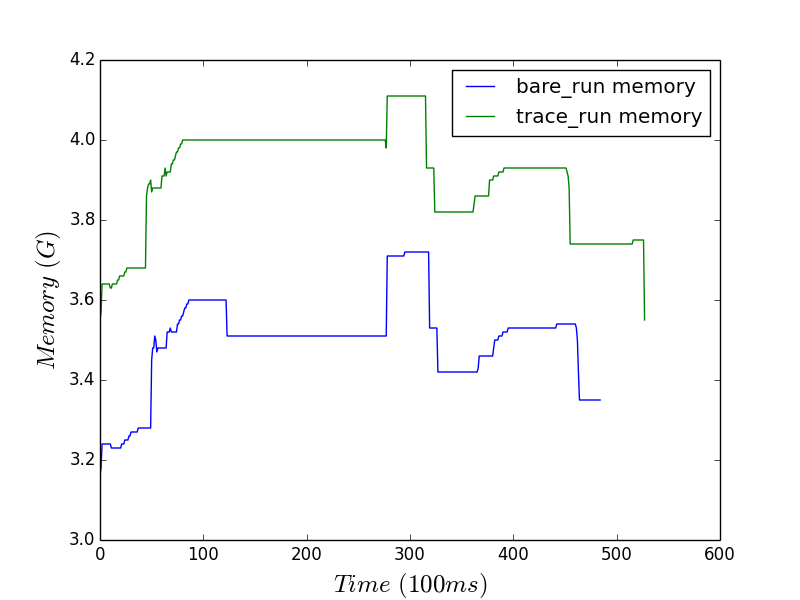
\includegraphics[width=1.0\linewidth]{ibench_memory_compare.png}
    \caption{Memory overhead with tracing.}
    \label{fig:ibench_memory_overhead}
\end{figure}

\begin{figure}[tb]
    \centering
    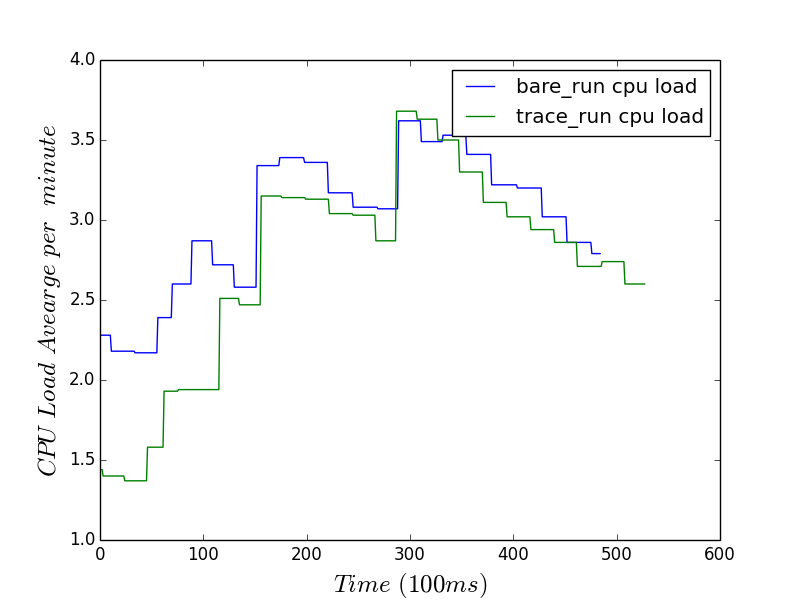
\includegraphics[width=1.0\linewidth]{ibench_cpuload_compare.png}
    \caption{CPU overhead with tracing.}
    \label{fig:ibench_cpu_overhead}
\end{figure}

\begin{itemize}
\item tracing overhead
	\begin{itemize}
	\item memory and CPU usage on top, while running ibench with and without our tracing enabled
	\item memory and CPU usage on top, while running the listed real world applications with and without our tracing enabled
	\item how much times it takes to filled the buffer we fixed 2G
	\item how many events recorded in the buffer
	\end{itemize}
\item number of edges and nodes in the graphs and portions of data the user need to examine to figure out the root cause.
\end{itemize}

\input{discussion}
\section{Related Work}
\label{sec:related-work}

While there is currently no system that can help users debug performance
issues in closed-source applications on proprietary macOS, several active
research topics are closely related.

\para{Event tracing.}
\begin{table}[ht]
\footnotesize
\centering
  \begin{tabularx}{\columnwidth}{l|XXX}
  \hline
Paradigm & Panappticon & AppInsight & \xxx\\
\hline
\hline
%User input & \mycheck & \mycheck & \mycheck \\
%Display update & \mycheck & \mycheck & \mycheck\\
Async calls & MessageQueue, & Upcall & libdispath\\
			& ThreadPoolExecutor &  & runloop \\
			&	&	&timer\\
IPC calls & \mycheck & \mycross & \mycheck \\
Batching & \mycross & \mycross & \mycheck \\
Data flag & \mycross & \mycross  & \mycheck \\
Wait-Wakeup & 4 primitives & Silverlight methods & system wide \\
%Fork & \mycheck & \mycorss & \mycross \\
%Interrupts &\mycross & \mycross &\mycheck\\
%Timeshare Maintain &\mycross &\mycross &\mycheck\\
%Syscall and backtrace
\hline
  \end{tabularx}
  \caption{Programming paradigms tracked.} 
  \label{table:paradigms}
\end{table}


Panappticon \cite{zhang2013panappticon} monitors a mobile system and uses the
trace to characterize the user transactions of mobile apps. Although it aims to
track system-wide events and correlate them without developer input, it supports
only two models of communication: work queue and thread pooling. AppInsight
\cite{ravindranath2012appinsight} instruments application to identify the
critical execution path in a user transaction. It supports the event callback
pattern, and does not trace across process or app boundaries.
Magpie~\cite{barham2004using} monitors server applications in Windows with the
goal to model the normal behaviors of a server application in response to a
workload. This model further helps detecting anomalies statistically. Magpie
requires a manual-written event schema for all involved applications to capture
precise request graphs, whereas \xxx has a simple, application-agnostic schema
for system-wide tracing and enables users to provide more application-specific
knowledge on demand.

Aguilela \cite{aguilera2003performance} uses timing analysis to correlate
messages to recover their input-output relations while treating the application
as a black box. XTrace, Pinpoint and \etc ~\cite{fonseca2007x, chen2002pinpoint,
chow2014mystery} trace the path of a request through a system using a unique
identifier attached to each request and stitch traces together with the
identifier. \xxx comes up violation patterns and does not assume the presence of
a unified identifier in closed-source, third-party applications, frameworks, and
libraries.


\para{Performance anomaly detection.}
Several systems detect performance
anomalies automatically. \cite{han2012performance, yuan2012conservative}
leverage the user logs and call stacks to identify the performance anomaly.
\cite{cohen2004correlating, saidi2008full, xu2009detecting, du2017deeplog}
apply the machine learning method to identify the unusual event sequence as an
anomaly. \cite{yu2014comprehending} generates the wait and waken graph from
sampled call stacks to study a case of performance anomaly.

These systems are orthogonal to \xxx as \xxx's goal is to diagnose an
already-detected performance anomaly. These systems can help \xxx by detecting
more accurately when a performance issue arises.

\section{Conclusion} \label{sec:conclusion}
Our key insight in this paper is that causal tracing is inherently
imprecise. We have reported patterns we observed that pose big precision
challenges to causal tracing, and built \xxx, a practical system for
effectively debugging performance issues in macOS applications despite the
imprecision of causal tracing.  To do so, it lets a user provide domain
knowledge interactively on demand. Our results show that \xxx effectively
helped us locate all root causes of the issues, including a bug in Chromium,
01 and incurred 12\% CPU overhead overall in its system-wide tracing.

\bibliographystyle{plain}
\bibliography{bib/biblio}

\end{document}

